\documentclass[]{article}

%packages
\usepackage{authblk} % Support for footnote style author/affiliation
\usepackage{graphicx} % Enhanced support for graphics
\usepackage{enumitem} % Extended management and customization for list settings such as enumerate, itemize and description
\usepackage{longtable}
\usepackage[backend=bibtex]{biblatex} % Sophisticated Bibliographies in LATEX
\usepackage[a4paper, total={6in,10in}]{geometry} % Flexible and complete interface to document dimensions
\usepackage[colorlinks=true, linkcolor=black, urlcolor=black, citecolor=black]{hyperref} % Enables hyperlinks

%variables
\graphicspath{ {./images/} } % ref to graphicx
\addbibresource{./references.bib} % ref to biblatex 

%opening
\title{Conceptual overview of the Logos network}
\author{Amar Čolaković, Angela Popa, Eugen Stoyanov}
\affil{LogosLabs}
\date{January 16, 2024}

\begin{document}
\maketitle

% ABSTRACT
\begin{abstract}
This document describes the concept of the \textit{Web3 sub0layer} Logos Network, a network that provides the Web3 infrastructure (layer-0 and layer-1 blockchain nodes) with a \textit{community provided and blockchain based autonomous computational core infrastructure}.
The necessity for a sub0layer and the impact it has on the Web3 and Web2 ecosystems is explained in this document, as well as the technical possibilities, challenges and approaches for building this network.   
This document represents a conceptual overview and not a technical documentation. It introduces the general idea of the Logos network and its implementation in the world wide web.

This concept is the foundation for the upcoming proof of concept (PoC) and for the technical documentation. 
With this approach, we aim to ensure that the Logos network not only has a solid theoretical basis, but is also realizable in practice and can be adapted to specific requirements.
This methodical approach should serve to evaluate the practicality and effectiveness of our concept with the highest possible accuracy.    
\end{abstract}

% CONTENT
\tableofcontents
\newpage

% INTRODUCTION
\section{Introduction}
The fundamental idea behind the Logos project is to establish an ecosystem, which shall provide the Web3 and Web2to3 communities with compute power generated by the community.
A lot of private PC-Hardware worldwide is either rarely used or in severe underuse. 
We are not talking about outdated workstations that are merely gathering dust in storage facilities, but rather daily used, up-to-date hardware, of which only a fraction of the overall potential gets utilized (Laptops, Home PC’s, Home Servers).

Currently the cost for computational resources supplied by the big Cloud-Services is barely affordable and presents a big challenge for small-scale ventures as they expand. (For a detailed analysis of cloud costs, read article 'The Big Cloud Exit FAQ'. \cite{david-hainemeier-hansson})
To counter this, the cost for compute-power shared by the \textit{Logos ecosystem} will be defined, under a strict and fair set of rules, by the community itself.

The core focus of Web3 and blockchain technology is decentralization and to eliminate the need of reliance in a third party.
Nowadays its evident that a large number of blockchain nodes, the backbone of decentralized structures, are hosted with big cloud providers (centralized structure (Azure, AWS, Google Cloud, ...)), thus defeating the purpose of true decentralization.
Services that provide a platform to easily deploy Web3 nodes rely on such big cloud providers, consequently relinquishing security, price and trust of those networks back to big companies.
Many who want to support those networks chose to use such services because of the complexity of node setups. 
The Logos network will aim to deliver a \textit{sub0layer} solution, so that every willing participant will be able to take part in a truly decentralized and community-secured infrastructure.

Nowadays community members with the required know-how and resources operate individual blockchain nodes. 
The easier, more secure and more elegant solution would be to use computational resources of those members, in order to  execute a genuinely trustless Web3-core-infrastructure. 
This infrastructure will be used as the computational foundation of the Web3 infrastructure.

Simply speaking, the \textit{Logos network} strives to create a community computer that belongs to everybody and no one.
An autonomous network to provide, receive and share compute-power.
A decentralized core computing environment, acting as an underlying layer (sub0layer) to a Web3 infrastructure (layer-0).

So called "layer-0" blockchains, which make up the Web3 infrastructure itself, are often hosted on conventional cloud services, reverting the infrastructure to a centralized one. 
Therefore a sub0layer is required, to secure and decentralize those hosted nodes again.  
This sub0layer shall also be applicable to Web2 based services to accelerate the migration to Web3.
It is important to encourage this migration, so that Web2 based applications/services can be secured by layer-0/layer-1 protocols, transforming those App's to DApp's of decentralized nature.

% FIGURE1
\begin{center}
	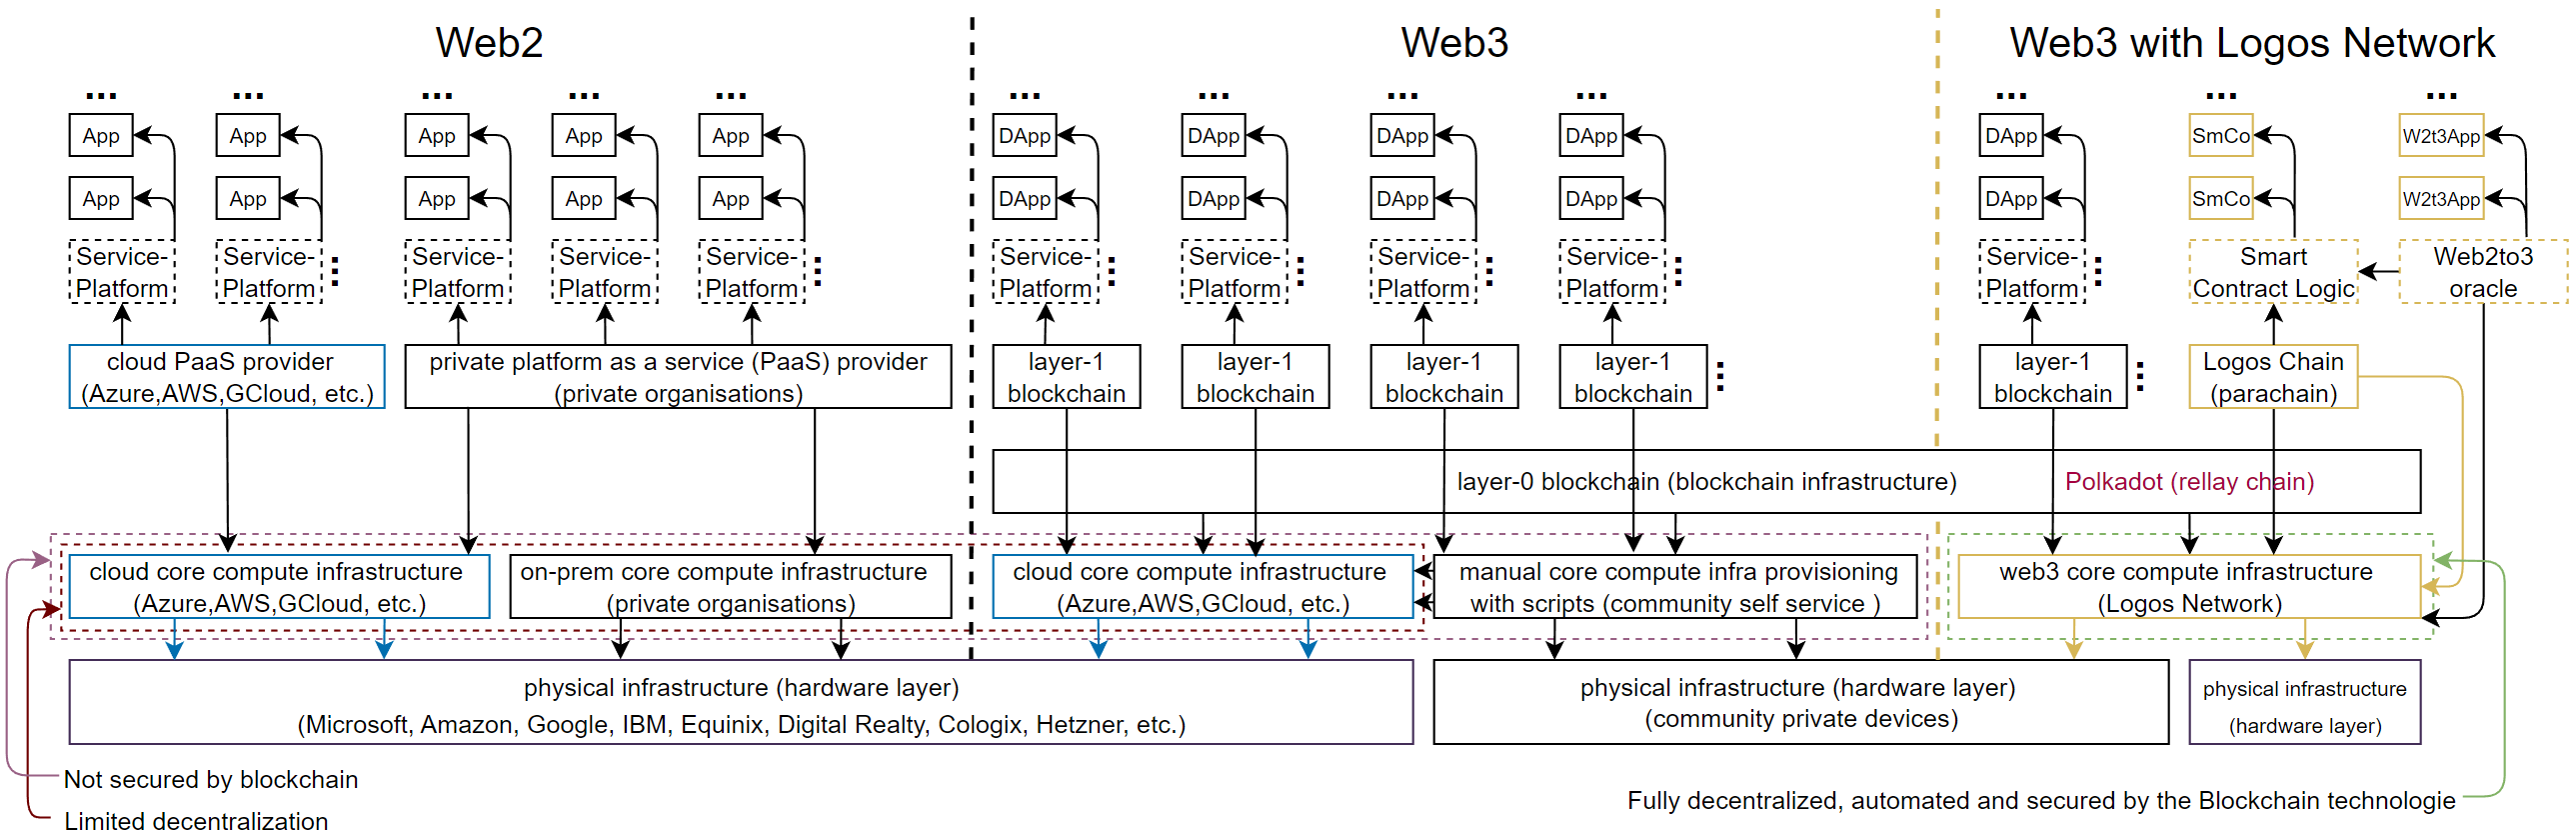
\includegraphics[height=5cm]{network-requirement}
\end{center}
\begin{center}
	Figure 1: Overview of a Web2 approach in comparison to Web3 and Web3 with a new security and compute layer and how the Logos network can enhance the Web3 infrastructure.
\end{center}

We aim to facilitate a computational core infrastructure which for the time being will be able to host Web2 based services prior to their migration to Web3. 
Therefore the Logos Ecosystem shall have a Web3 service tasked with providing a Web3 core infrastructure for layer-0,1 blockchains. 
This Web3 service will work side by side with two distinct Web2based applications, which themselves will be migrated to Web3, once the conditions are met.
These two services will be partially integrated into the blockchain, so that they can access and interact with the network.
A bridge-like "communication channel" will be developed for these services and the blockchain to simplify future migrations.

After successful release of Logos network 1.0 the sudo privileges, and thereby the only means to act upon the network structure, will be relinquished to the community, who will be able to take advantage of those privileges under a set of governance systems. 

% NETWORK
\section{Network}
The Logos network will provide a secure \textit{Web3 core compute infrastructure} the resources of which are provided by the community. 
The infrastructure will be defined, secured and executed by a blockchain.
The Logos network will consist of three main components: the \textit{DVCI (Distributed Virtual Computing Infrastructure)}, the \textit{Logos chain} and a \textit{Network Gatekeeper}. 

The DVCI will act as a "data center" where a blockchain will be utilized to ensure the security of operations.
The DVCI combines community-provided resources and dedicates those resources to "servers" with virtual environments.
Although this DVCI will primarily be aimed at enhancing the Web3 core infrastructure, it will also be applicable to Web2, due to the present need of a Web2to3 migration platform.
This DVCI will not be intended for low-latency Web2 applications (e.g. financial institutions, stock markets, critical real-time systems, ...), hence why the use cases for the Logos network will have to be strictly defined, to ensure an optimal usage of all the different computational components.  

A blockchain is simply a chain of data-blocks.
Each data-block contains a list of transactions, securely stored on a multitude of nodes. 
All the information stored within those data-blocks is truthful and tamper-proof.
This type of technology and the implementation of a \textit{Smart Contract Logic} allow for the existence and operation of the aforementioned DVCI.

The network gatekeeper will ensure that each infrastructure component (existing and future) complies with all security protocols, handle the communication between the DVCI and the blockchain and also transfer new instructions/configurations to the underlying blockchain.

% FIGURE2
\begin{center}
	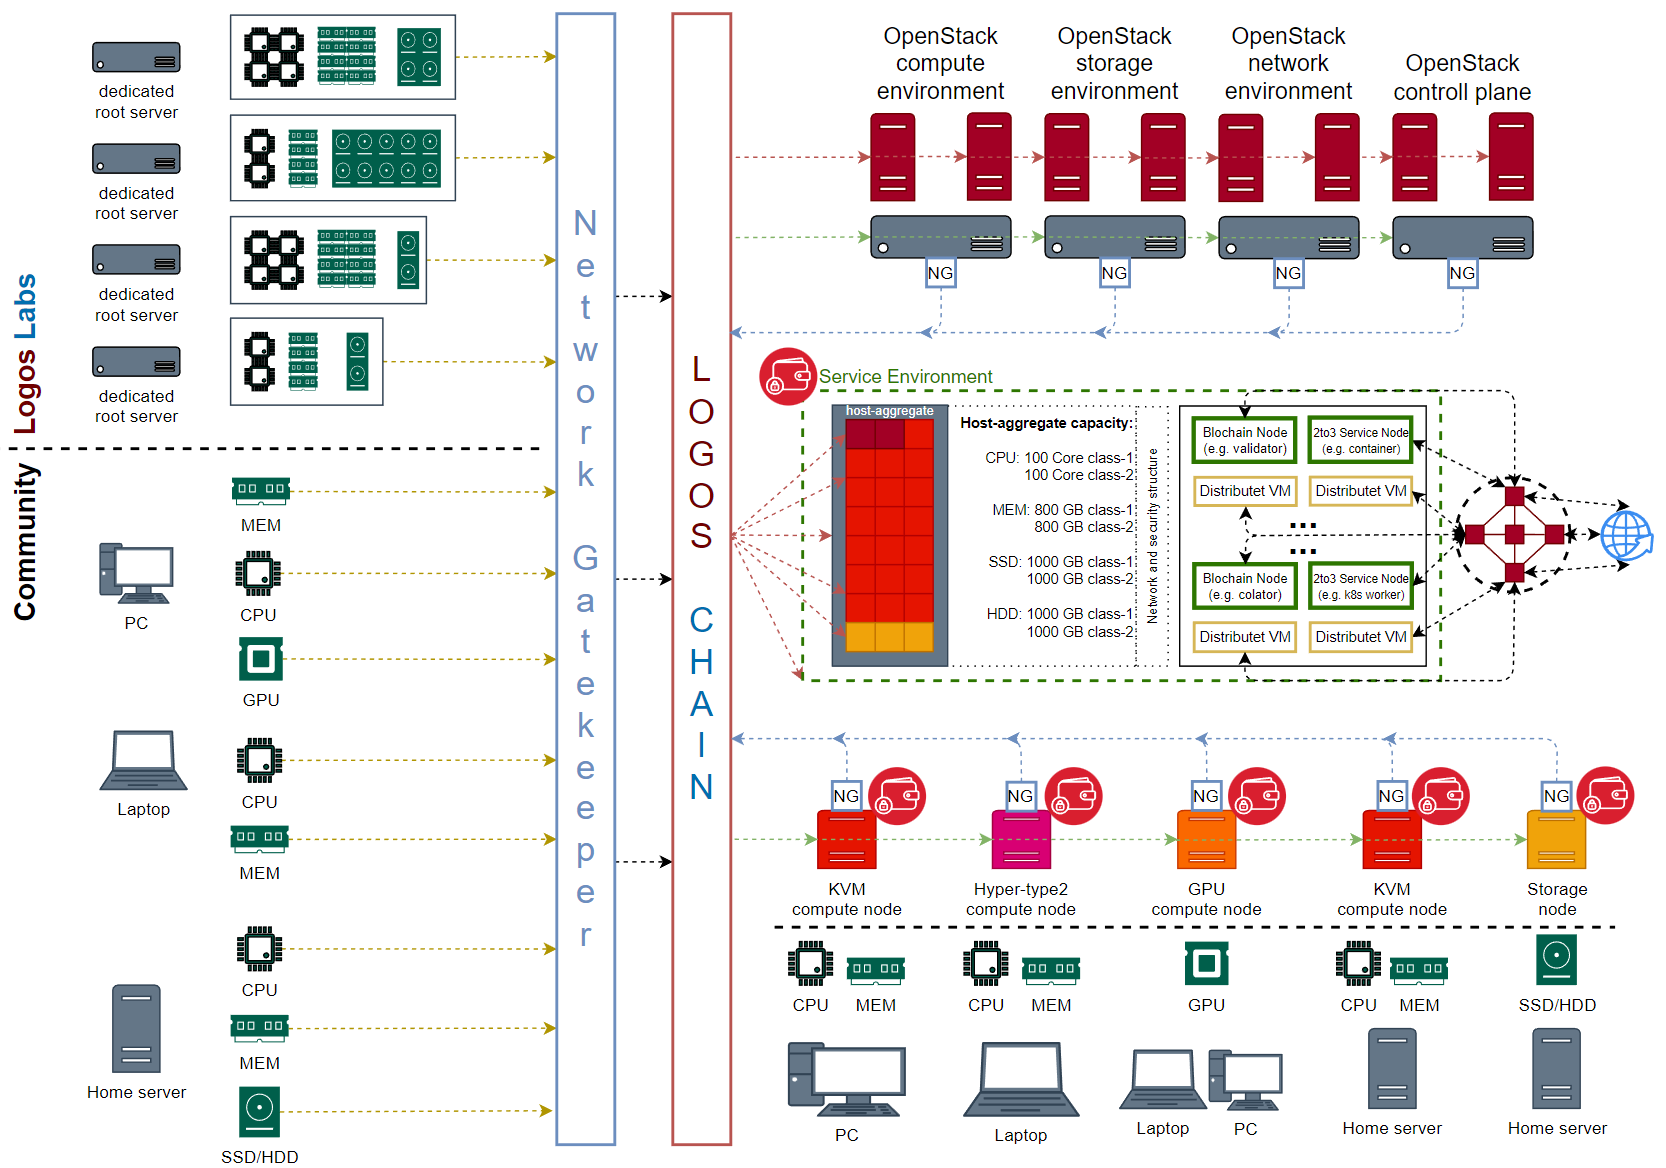
\includegraphics[height=10.5cm]{logos-network}
\end{center}
\begin{center}
	Figure 2: Conceptual overview of the Logos network and its benefits.
\end{center}

The development of the Logos network will incorporate, in addition to in-house developments, a variety of existing technologies, tailored to the specific requirements of this type of network.
The main aspects which define the philosophy of the Logos ecosystem are: IaC (Infrastructure as a code), autonomous solutions, security and decentralization.

% DISTRIBUTET VIRTUAL COMPUTING INFRASTRUCTURE
\subsection{Distributed Virtual Computing Infrastructure}
Big data centers these days can provide centralized computational infrastructures with ease.
Because the DVCI is based on a decentralized approach, a variety of different issues will have to be addressed (e.g. network latency, virtualization in distributed environments, aggregated computation, ...).
A cloud infrastructure, as DVCI aims to be, ultimately exists to productively manage Web2 and Web3 services, that is why response time is a crucial factor. 
Response time being the duration it takes for a request to be processed and returned to the requester.
It is a unit of measurement for the "rate" of a system. 
It is important to note that this response time is not only defined by intern processes but also affected by external factors (connection quality, hardware performance, local conditions, ...).

A crucial component of such an infrastructure is a low-latency software defined network (SDN) to achieve acceptable response times.
The challenge of such an SDN is, to connect all participants in a manner so that their resources can be accessed by virtual compute environments via "resource-pools".
Each global region shall have its own computational network to ensure optimal resource management.
In addition to \textit{computational networks (CoN)} there shall be two additional network groups, namely \textit{service networks (SeNe)} and \textit{regional bridge networks (RBN)}.
SeNe's will be used to divide resources into global regions, whereas RBN's will establish the connection between aforementioned regions.

Virtualization in distributed environments is another crucial part of this DVCI.
By utilizing Hypervisor technology, especially type-1 Hypervisors, it is possible to create a virtual environment that can access hardware "directly" without an OS-layer.
Its important to mention that those environments can be fully isolated using different methods.
Even in case a user has root privileges, his access to KVM resources can be limited by certain configurations and security measures.
Since not every resource provider's OS is capable of running type-1 Hypervisors, the type-2 Hypervisor will also be utilized.
The only downside being the increase of computational duration, due to the OS-layer.
By using OpenCL (Open Computing Language) and ROCm (Radeon Open Compute Platform), GPU virtualization (for use cases requiring this specific type of resource) can also be accomplished.
Due to not every provided hardware being of same quality, resources will have to be divided into classes (by efficiency, compute-periods, volume of processable date, ...) in order to task them with fitting services.

% FIGURE3
\begin{center}
	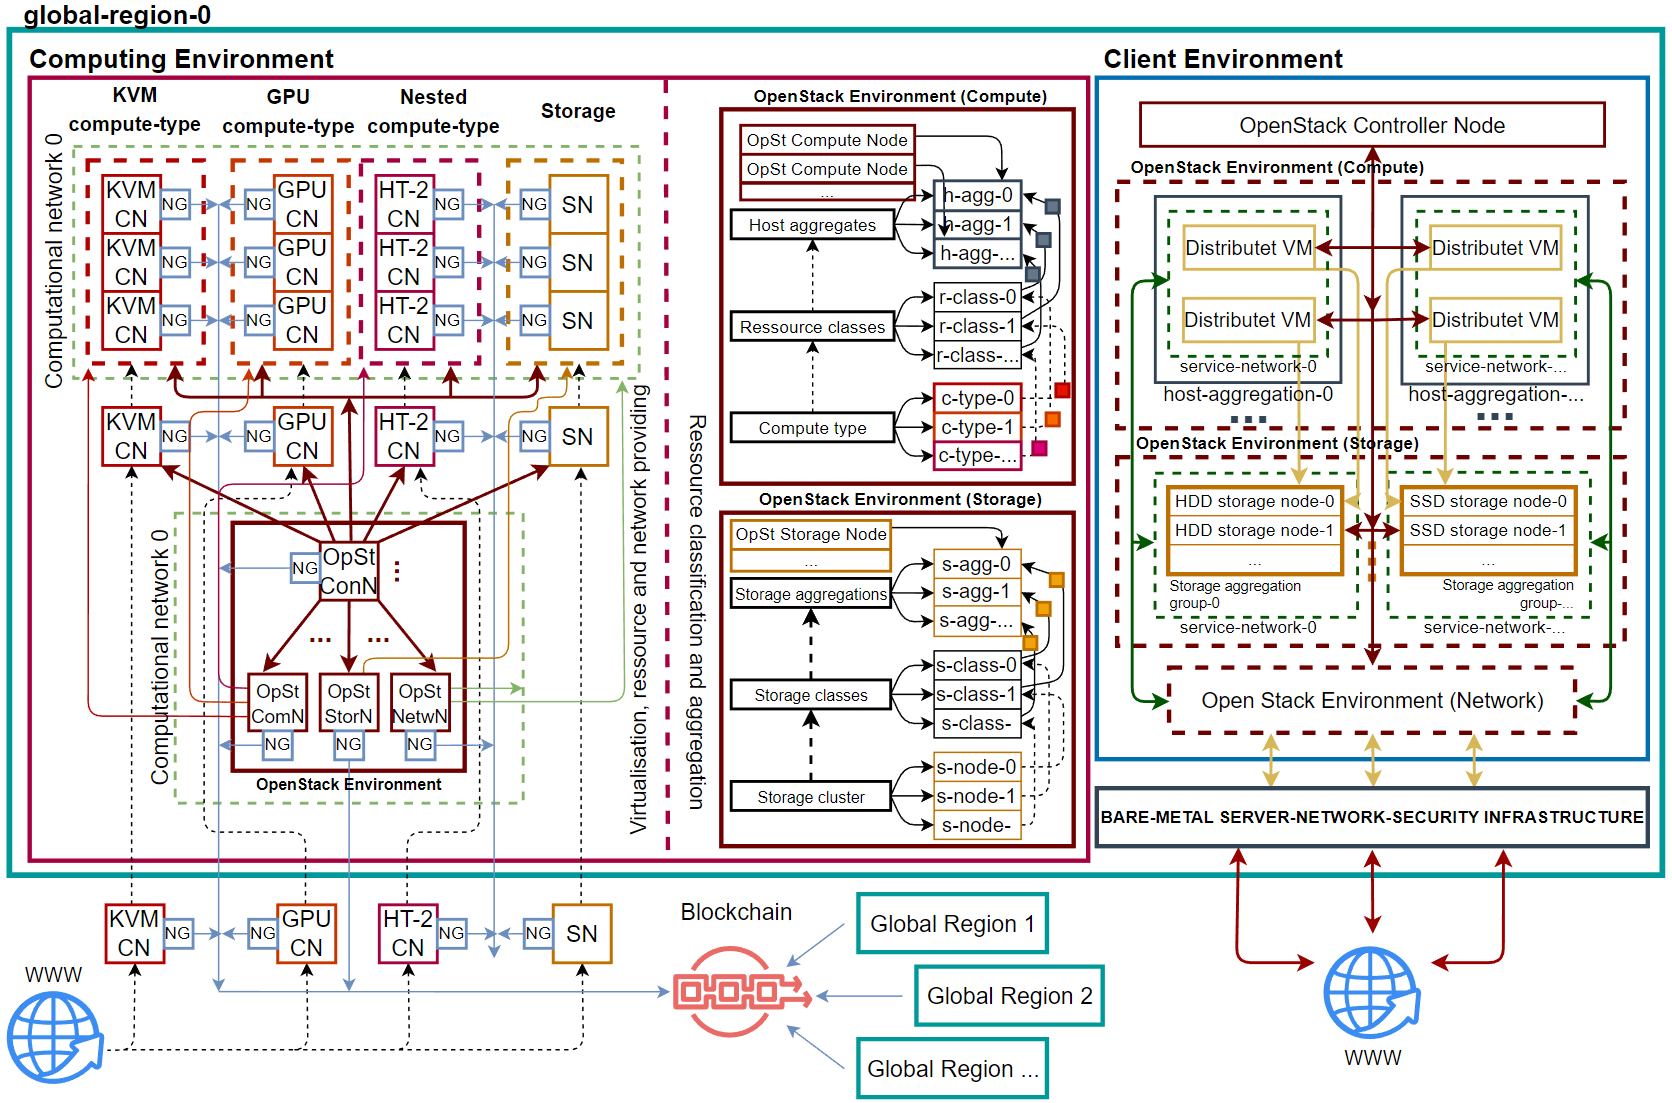
\includegraphics[height=10cm]{dvci-arch-overview}
\end{center}
\begin{center}
	Figure 3: High-level overview of the Distributed Virtual Computing Infrastructure and its components.
\end{center}

Each global region gets assigned a minimum of four dedicated root servers with an \textit{OpenStack environment}.
This OpenStack environment will be subject to the \textit{environment controle node (ECN)}.
The ECN consists of an OpenStack controller node and the corresponding network gatekeeper components. 
After the creation and configuration of suitable service environments (in the OpenStack environment) they will get assigned so called \textit{host aggregates}. 
Besides their own dedicated computational resources, the host aggregations will also get distributed resources assigned to them, in order to run corresponding VM's/containers.
OpenStack offers functionalities in the field of IaC and automation, which will be used to improve accessibility and autonomous functions of the infrastructure.
Each global region will have its own DVCI instance, which means every DVCI will be able to operate independently.
The communication between all existing DVCI's will be carried out via RBN's and Geo-clustering. (chapter 2.1.4)

\textit{Every single component of a DVCI should be build, secured, configured and supervised by the blockchain.} (chapter 2.2)

% ARCHITECTURE AND COMPONENTS
\subsubsection{Architecture and components}
The DVCI can also be laid-out as a reference model.
Layer-0 is the physical layer.
This layer combines dedicated root servers and distributed community hardware. 
Layer-1 on the other hand, is the layer, where basic hosting, virtualization, network and security infrastructures will be set up. (host-OS, host-Firewall, Hypervisor, networking and load balancing, failover mechanism, ...).
Whereas layer-2 (computing environment) will be the one providing a cloud infrastructure for the OpenStack environment.
Layer-2 will also be responsible for categorizing and bundling of provided computation resources.
Within the last layer a.k.a client environment (layer-3) different service environments will be generated (cloud-service level) and configured.

% FIGURE4
\begin{center}
	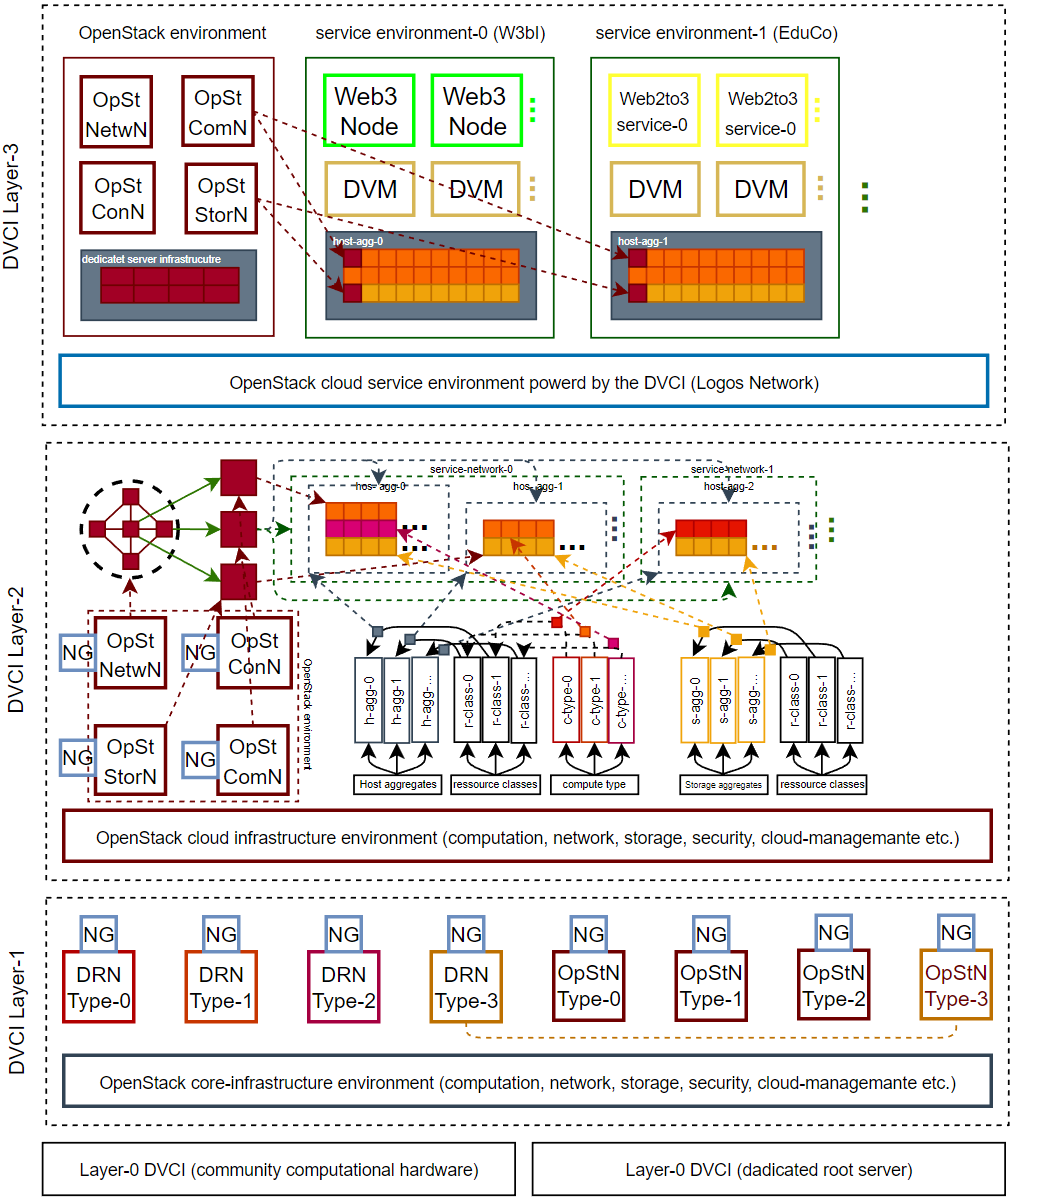
\includegraphics[height=15.4cm]{dvci-layers}
\end{center}
\begin{center}
	Figure 4: Overview of a Distributed Virtual Computing Infrastructure as a reference model.
\end{center}

% GLOBAL REGION
\textbf{Global Region}: 
Computational resources will be divided into geographic (global) regions.
The idea behind this division is to ensure optimal networking, virtualization and resource management on a local scale.
The amount of such regions will heavily depend on the network components' overall global latency, and will increase if lower response times are needed.
\newline

% DEDICATETD ROOT SERVER
\textbf{Dedicated Root Server:}
These servers will be tasked with providing an OpenStack environment for the DVCI in a global region.
Every global region, as mentioned earlier, will have four dedicated root servers assigned to them in order to facilitate a server failover mechanism.This will enable the migration of a service to another server, in case of hardware malfunction.
A reliable method in "high-availability" and "disaster recovery", is to physically distance data centers from each other. 
Specifically the "active/passive failover" mechanism will be used.
The advantage of this type of mechanism is, that standby-servers use only a small amount of computational resources, unless a service-migration has to be undertaken. 
All root servers will operate a host-OS under strict security precautions. 
The form of bare-metal network and LB-infrastructure will depend on the quality of the data center network infrastructure.
\newline

% REGION ENVIRONMENTS
\textbf{Region Environments:}
The term region environments is used as a collective term for layer-2 and layer-3. 
Region environments will separate the DVCI into phases, depending on field of activity, thus simplifying configuration management and oversight.
Each global region will consist of a computing environment and a client environment. 

\begin{enumerate}[label=\textbullet]
	% COMPUTING ENVIRONMENT 
	\item\textbf{Computing Environment:}
	The computing environment(layer-2) or back-end phase will take on layer-specific actions in managing, connecting and securing the DVCI. 
	Besides providing a platform for the OpenStack environment, this layer-2 will also bundle provided resources, by resource class, into host-aggregates and deliver said resources to the service layer.  
	
	% CLIENT ENVIRONMENT
	\item\textbf{Client Environment:} 
	The client environment will be the "execution-layer" for the DVCI and act as the access point for cloud services (W3bI, EduCo, SciCo, ...). 
	Client environments will be created in this layer (via OpenStack) and aforementioned host-aggregates distributed to \textit{DVM's (Distributed Virtual Machines)}.
	Virtual environments will be isolated through service networks, to ensure secure separation of different services. 
\end{enumerate}

% FIGURE5
\begin{center}
	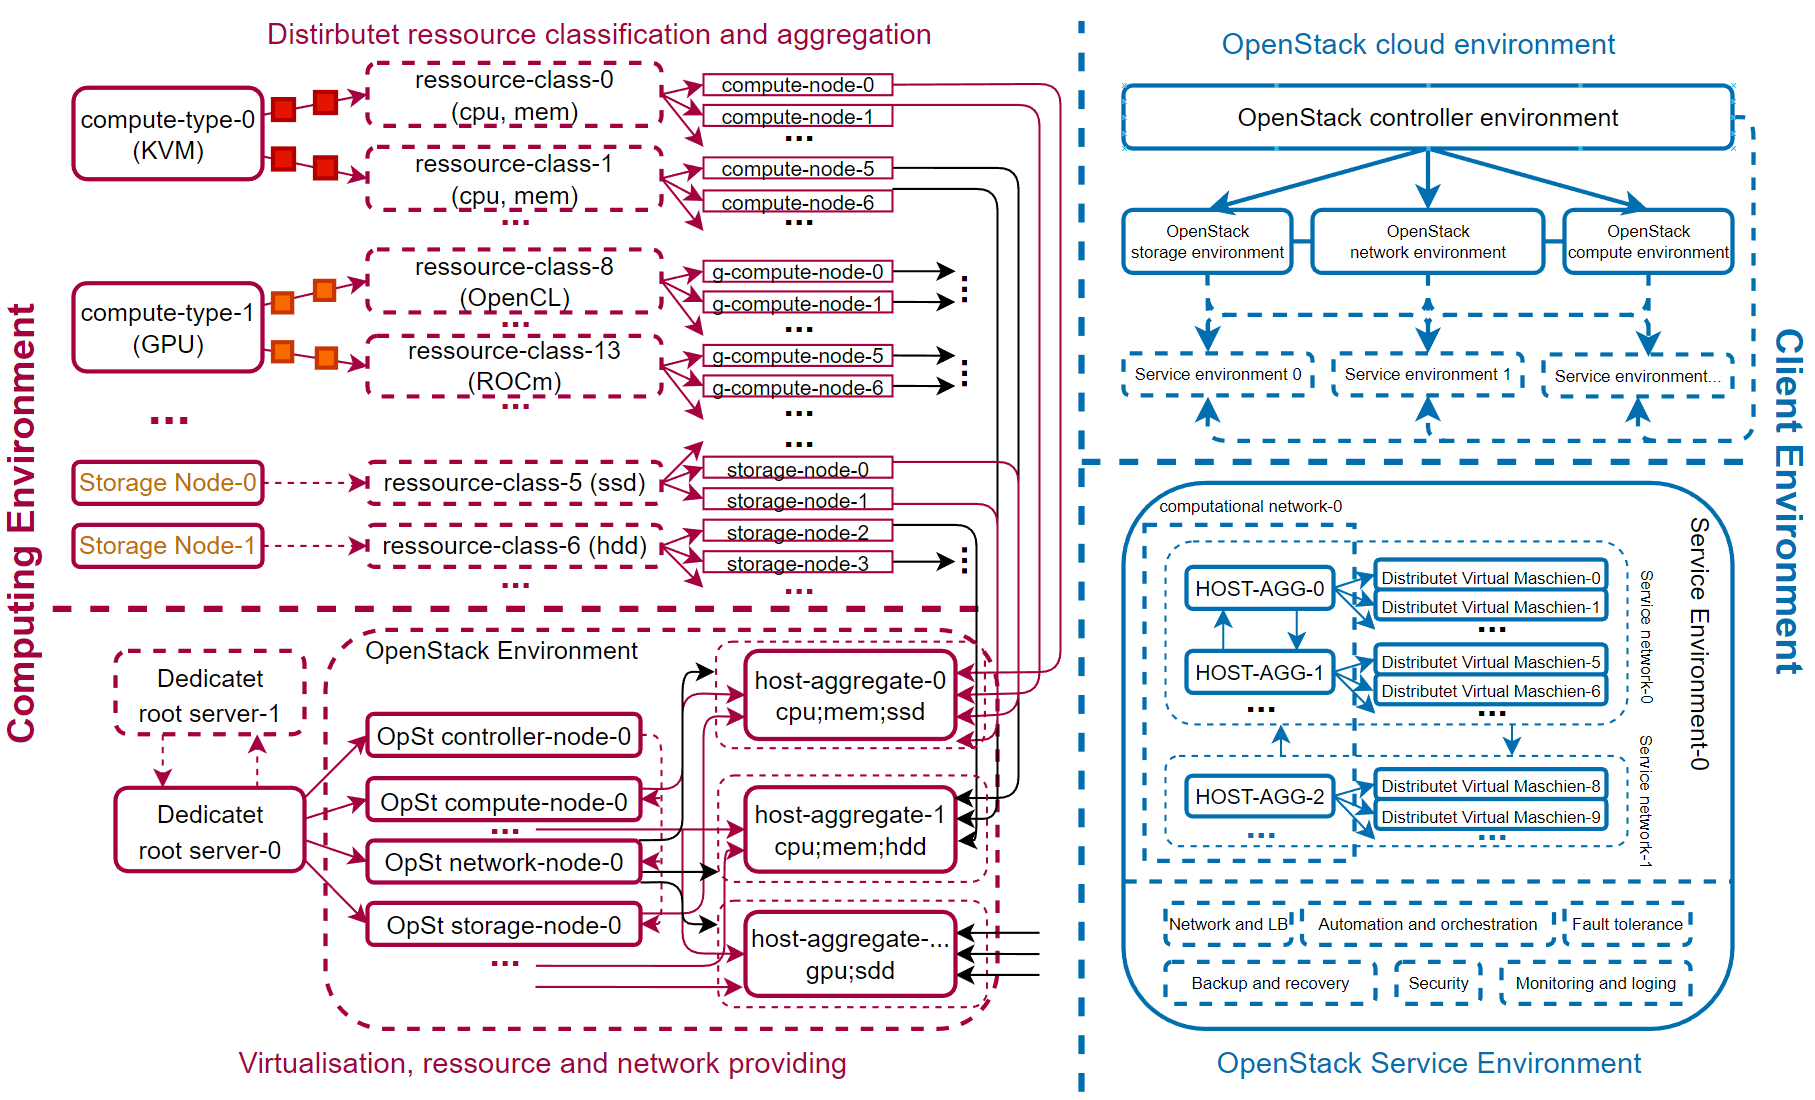
\includegraphics[height=9cm]{region-environments}
\end{center}
\begin{center}
	Figure 5: High-level overview of region environments and their workflows.
\end{center}

% OPENSTACK ENVIRONMENT
\textbf{OpenStack Environment:}
OpenStack is a comprehensive cloud-infrastructure solution, that provides a wide variety of tools and resources for the deployment, scaling and management of virtual environments and other cloud resources. 
OpenStack allows for the creation of networks, able to meet the requirements of cloud-computing infrastructures. 
It also supports different virtualization technologies, storage and network solutions.

The OpenStack architecture used for the Logos network will consist of four Node-types playing different roles.
The first type (controller node) will host the main OpenStack services required for the DVCI.
The second type (compute node) will take on the execution of VM's (DVM's).
The third type (storage node) will facilitate storage and retrieval of data.
The fourth and last type (network node) will coordinate network resources, configure network topologies as well as enable and manage communication channels between the VM's (DVM's) and external networks. 
Each OpenStack environment will have to retain at least two nodes of each type, for load-balancing and high-availability to function uninterrupted.
The choice if a node will be a physical server or a virtual machine will depend heavily on the service type and the computational requirements.
For a more comprehensive understanding of OpenStack, see \cite{OpenStackDoc-design}.

\begin{enumerate}[label=\textbullet]
	% CONTROLLER NODE
	\item\textbf{Controller Node:}
	In an OpenStack environment the term controller node is associated with the key component of the OpenStack-system, serving the purpose of management different OpenStack services.(Keystone, Glance, Nova and Neutron (control components), Heat, ...). 
	For detailed insights into the control-plane design, refer to \cite{OpenStackDoc-control}
			
	% COMPUTE NODE	
	\item\textbf{Compute Node:}
	Compute nodes, included in the OpenStack system, will be responsible with the distribution of computational resources and the execution of the DVM's. 
	The most important component operated by a compute node is "Nova" (OpenStack compute service).
	Every node should have its own Hypervisor (type1) to enable the creation and execution of VM's (DVM's). 
	For further information on compute architecture, see \cite{OpenStackDoc-compute}. 
	The approach of node-type separation on different physical servers is aimed at improving the virtualization efficiency.

	% STORAGE NODE
    \item\textbf{Storage Node:}
    These nodes will provide storage space in form of block storage (Cinder) and object storage (Swift). 
    For a deeper understanding of the storage architecture, review \cite{OpenStackDoc-storage}.
    Future research will determine if the efficiency of a single physical server hosting both storage and compute node is acceptable. 
  
	% NETWORK NODE 
	\item\textbf{Network Node:}
	A network node (physical server or virtual machine) will be responsible for network traffic, run network services (Neutron, Octavia, Designate) and define the network topology inside an OpenStack environment. 
	This node will play a vital role in the communication between different OpenStack environment components and external networks. 
	To delve deeper into the topic of the network architecture, see \cite{OpenStackDoc-network}. 
	If network nodes will have to be set up on separate physical servers or could be combined with compute/storage nodes, will also have to be determined in future research. 
\end{enumerate}

Future research (PoC) shall also define the amount of physical servers to be used per global region as well as the advantages and disadvantages of different server configurations (combined nodes or single node servers).
\newline

% DISTIRBUTET RESSOURCE NODE
\textbf{Distributet Ressource Node:}
This type of node will connect distributed resources to the DVCI. 
\textit{Distributed resource nodes (DRN's)}, from a simple perspective, would have to be PC's and home-servers, from the networks perspective however, they will be virtual compute/storage nodes.
Compute nodes will have the option to commit to SLA's (service-level-agreement) therefore increasing the DVCIs control over the provided resources.
DRN's will have to be categorized by the provided resource type (CPU, RAM, GPU, HDD/SSD).
Each DRN will also be equipped with its own client network gatekeeper.
Subsequent to the separation into global regions, by the network gatekeeper, the DRN's will be connected to a virtualization network and assigned host-aggregates via the OpenStack environment.
Each provider (of distributed resources) will have to be a separate, isolated environment. (SELinux, AppArmor, Cgroups, Libvirt Access Control, GPU-passthrough, ...) 
This should enable providers to lend resources to the network while using the remainder for their local applications. 
In order to deliver distributed resources securely and efficiently several factors will also have to be accounted for (network connection, network latency, compute-times, fail-safe measures).  

\begin{enumerate}[label=\textbullet]
	% KVM COMPUTE NODE
	\item \textbf{KVM Compute node:}
    KVM compute nodes will be tasked with providing the network with CPU's and RAM. 
    This type of node will only be applicable to hardware capable of virtualization (KVM).
    Contrary to OpenStack compute nodes, KVM compute nodes will only be equipped with "libvirt" used by NOVA, not the full service. 
			
	% HYPER-TYPE2 COMPUTE NODE
	\item \textbf{Hyper-Type2 Compute node:}
	As is the case with the KVM compute node, the Hyper-type2 compute node will also be tasked with providing CPU and RAM, but with a type-2 Hypervisor.
	The necessity of this type of node arises from not every operating system being able to support type-1 Hypervisors.
	(PoC: Efficiency of different types of virtualization environments needs to be analyzed) 
	
	% GPU COMPUTE NODE
	\item \textbf{GPU Compute node:}
	The GPU compute node will be tasked with providing GPU's.
	Based on the type of chip architecture (NVIDIA, AMD) the provided resources will have to be collected by the network by using either OpenCL or ROCm.
	Like the previous types of nodes, the GPU compute node will also be managed and configured via an OpenStack environment. 
		
	% STORAGE NODES
	\item \textbf{Storage node:}
	Storage nodes (full OpenStack node) will be tasked with providing data storage. 
	These nodes should be bound by at least a 24-hour SLA and have server-like hardware requirements, to ensure more efficient data management within the DVCI.  
\end{enumerate}

% VIRTUALIZATION AND CLUSTER COMPUTING
\subsubsection{Virtualization and cluster computing}
A couple of different hardware virtualization technologies exist nowadays. 
The task at hand is to choose the most suited for a distributed virtualization environment. 

The physical node of type-0 will be the provider (of computational power) on a Linux Kernel, which enables the utilization of the KVM technology. 
In this case the type-1 Hypervisor can be used to directly access the hardware without an intermediate layer. 
This approach is only possible on Linux based systems.
Most Windows based systems on the other hand, are not capable of type-1 Hypervisor features.
Possible solutions for these types of systems would a type-2 Hypervisor (nested) approach or the exclusion of those systems from CPU and RAM pools (only GPU).
(PoC: Efficiency of nested virtualization against the GPU-only approach will be compared)

% FIGURE6
\begin{center}
	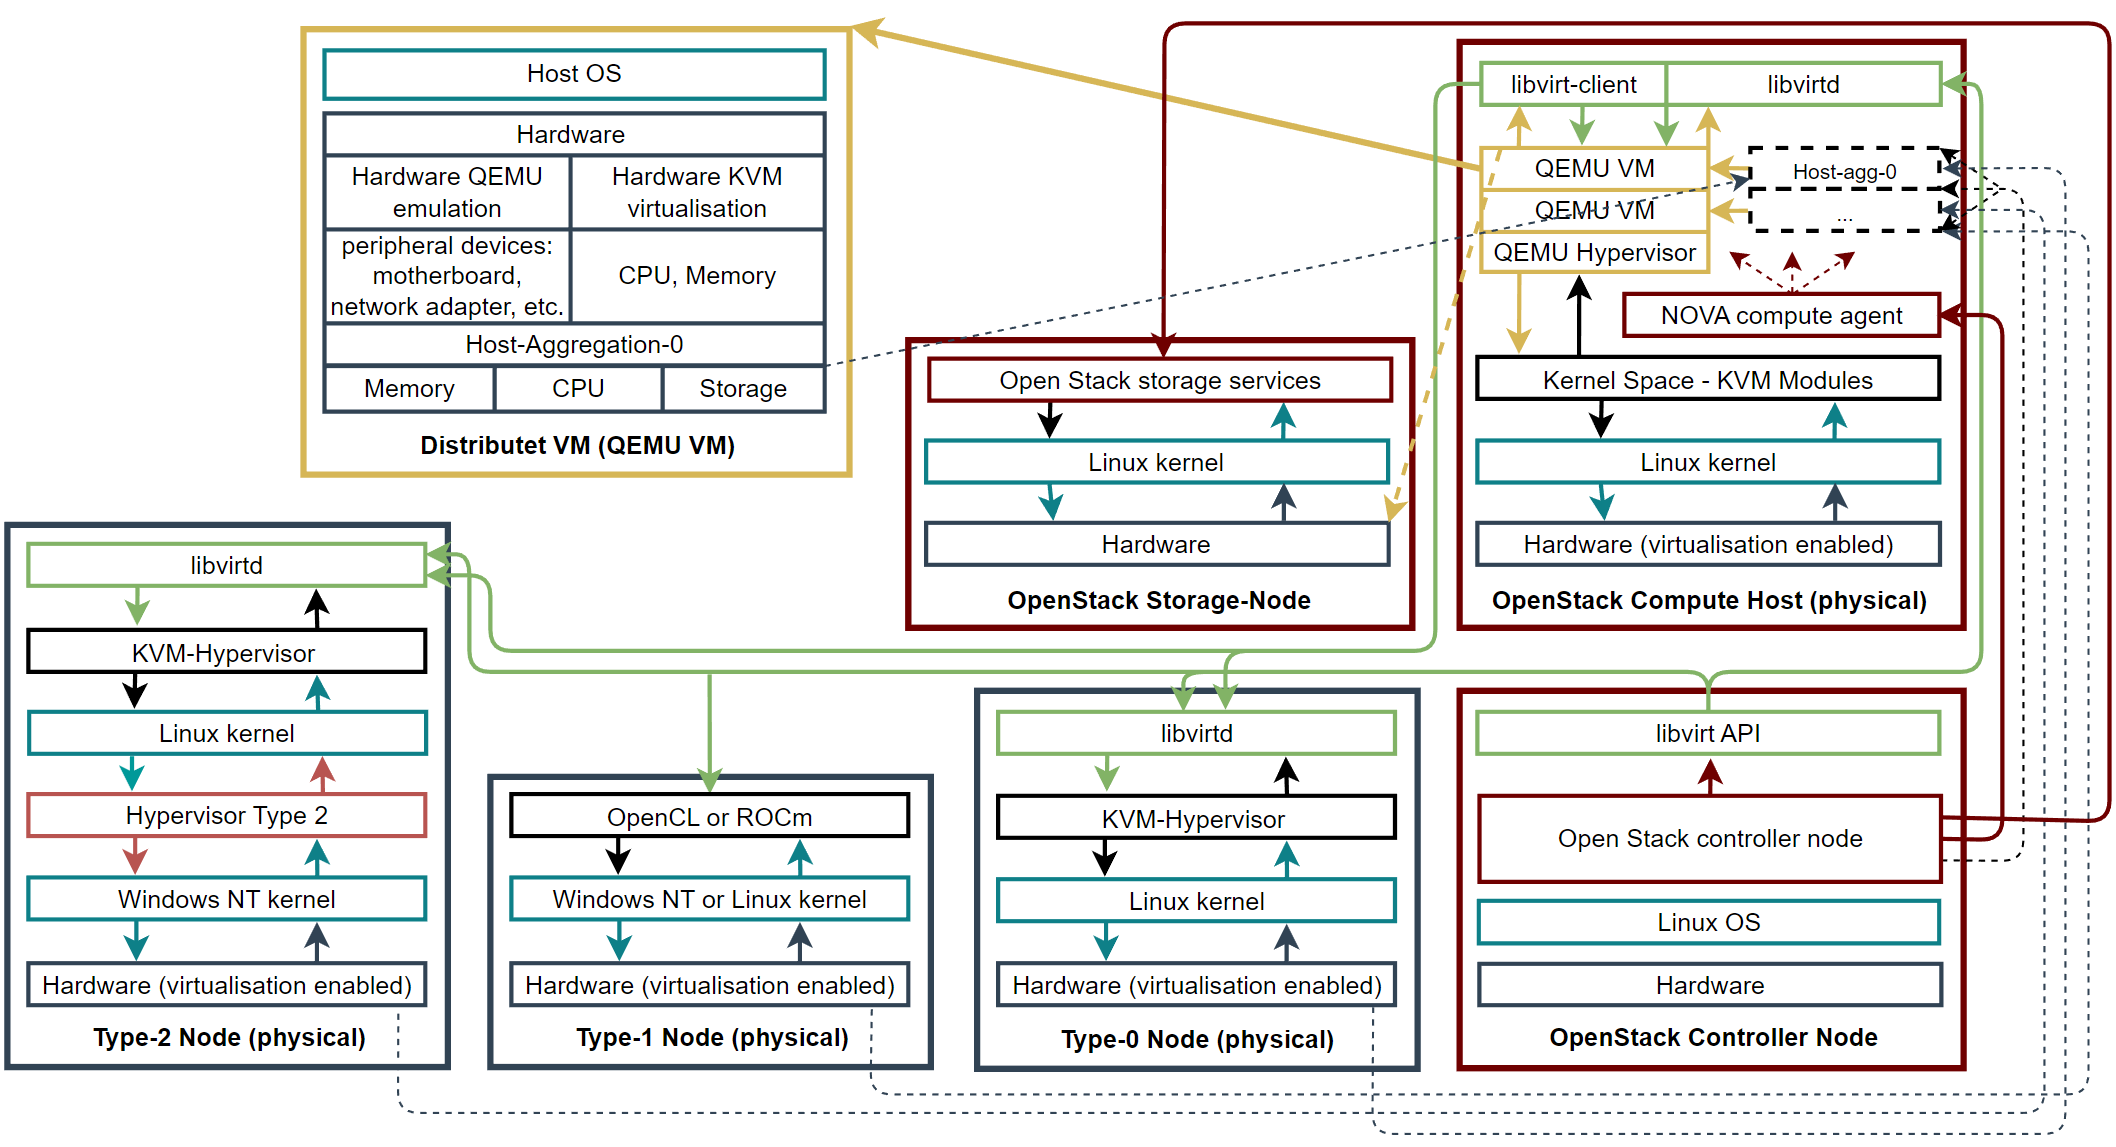
\includegraphics[height=8cm]{virtualisation-overview}
\end{center}
\begin{center}
	Figure 6: High-level overview of virtualization and cluster computing.
\end{center}

% HYPERVISOR
\textbf{Hypervisor}:
The term hypervisor is used to describe a type of computer software, firmware or hardware responsible for the virtualization of computational resources.
Hypervisors act as a transitional layer between physical hardware and future guest operating systems.
Two types of Hypervisors (type-1, native or bare-metal and type-2 or hosted Hypervisors) exist and are implemented in different ways. See documentation \cite{Wikipedia-Hypervisor}.  

\begin{enumerate}[label=\textbullet]
	% TYPE-1 HYPERVISOR 
	\item\textbf{Type-1, native or bare-metal Hypervisors:}
	These Hypervisors (hardware) run directly on the host's hardware, control the hardware and manage guest operating systems. 
	The type-1 Hypervisor to be used for the provision of distributed virtualization environments, based on Linux systems, is the KVM Hypervisor. 
		
    % TYPE-2 HYPERVISOR 
	\item\textbf{Type-2 or hosted hypervisors:}
	Type-2 Hypervisors (software) run on a conventional operating system (Windows, Debian/GNU, macOS, ...) just as other computer programs do.
	This type of Hypervisor enables the virtualization of resources at the software level without the need for special hardware. 
\end{enumerate}

% KVM & QEMU
\textbf{KVM and QEMU}:
The Kernel Virtual Machine is a technology and a Linux kernel extension that makes it possible to support hardware virtualization, allowing the kernel to act as a type-1 Hypervisor.
For a more comprehensive understanding of the KVM technology, see \cite{KVMDoc}.
The Quick Emulator or QEMU (type-2 Hypervisor) is a virtualization software that uses various virtualization techniques to virtualize (guest) operating systems on non-identical hardware.
For a deeper understanding of QEMU, review \cite{QEMUDoc}.
QEMU is very often used in combination with KVM as backend.
While KVM provides the resources such as CPU and memory, QEMU emulates the required peripheral devices such as network cards, motherboard, etc.
\newline

% LIBVIRT
\textbf{libvirt}:
Libvirt is a set of libraries and a toolkit that serves as an interface for managing various virtualization technologies and Hypervisors. 
It is designed to facilitate the management and automation of virtualization tasks and provides a unified API for interacting with different virtualization platforms.
For a thorough description of the libvirt project, reference \cite{libvirtDoc}.
The libvirt project can be used independently with its CLI-tool virsh. 
However, libvirt is primarily intended to be used via the OpenStack environment.

\begin{enumerate}[label=\textbullet]
	% LIBVIRT APIs
	\item\textbf{libvirt-APIs:}
	The libvirt-API is a central component of libvirt. 
	It enables standardized interaction with a variety of Hypervisors (KVM, QEMU, Xen, Hyper-V, ...), which facilitates the development of virtualization management tools and applications. 
	Libvirt-API is actually just a collective term, as it offers a variety of APIs. 
	For further informations on libvirt-APIs, see \cite{libvirtDoc-api}.
	
	% LIBVIRT DAEMON	
	\item\textbf{libvirtd:}
	The libvirt daemon is responsible for receiving instructions from the libvirt-api or the libvirt-client and forwarding them to the Hypervisor. 
	For detailed insights into the libvirt daemon, refer to \cite{libvirtDoc-daemon}. 
	
	% LIBVIRT CLIENT
	\item\textbf{libvirt-client:}
	The libvirt client allows direct access to the libvirt daemon on remote hosts, which results in the OpenStack Compute Nodes being able to access and manage the remote resources efficiently. 
	For a better understanding and the utilization of the libvirt-client, consider  \cite{libvirtDoc-remote-support} and \cite{libvirtDoc-connection-uri}.
\end{enumerate}

% OPENCL & ROCm
\textbf{OpenCL and ROCm}:
OpenCL provides a cross-platform API for heterogeneous systems, while ROCm is a platform from AMD that relies on various open standards and programming interfaces to utilize the computing power of AMD GPUs and accelerators. 
Both technologies are designed to facilitate parallel programming on heterogeneous systems.
To delve deeper into the topic of the OpenCL and ROCm project, see \cite{OpenCLDoc} and \cite{ROCmDoc}.
The basic idea behind the use of OpenCL and ROCm is to write so-called kernels to be executed on remote graphics cards.
These kernels are then send over the network to the graphics card, which performs the calculations and sends the results back to the application system.

This can be useful if the computing power of remote GPUs is to be used without the GPU being physically installed on the same system as the application. 

% STORAGE AND VOLUME CLUSTERING
\subsubsection{Storage and volume clustering}
A distinction must first be made between ephemeral and persistent storage in the provision of storage resources in a DVCI.
The difference between ephemeral and persistent storage lies in the way data is stored and handled, especially in the context of virtual machines or cloud instances. 
Simply put, ephemeral storage is temporary, while persistent storage is used to store data permanently.
The persistent storage will be provided in the form of object or block storage via the distributed storage nodes (DRN's), where ephemeral storage will be provided through the dedicated root servers. 

Block and object storage are two different approaches to storing data, and they are used depending on the requirements.
\newline

% BLOCK STORAGE
\textbf{Block Storage:}
Block storage is a type of storage that organizes data in blocks, where each block is considered a separate unit. 
Block storage is flexible and can be used for various use cases, including being used as hard disks for virtual machines or for storing databases. 
\newline
	
% OBJECT STORAGE	
\textbf{Object Storage:}
Object Storage organizes data in objects that are assigned a unique identifier (ID). 
In addition to the actual data, each object also contains metadata and a unique address that can be used to access it.
Object storage is highly scalable and is well suited for large volumes of unstructured data, such as those used in cloud storage solutions or content delivery networks (CDNs). 
\newline

In summary, block storage is suitable for use cases where you need file system access, such as operating systems or databases that rely on hard disks.
Object storage, on the other hand, is suitable for large amounts of data, such as media files, backups and other unstructured data.
Both types of persistent storage will be provided within the DVCI.

It is also important to differentiate between storage types and file systems.
Fundamentally the DVCI will provides storage (block and object) but depending on the use case different file systems (IPFS, NFS CephFS, ...), will be used in the interaction with that storage.

The storage (persistent) is to be provided on a technical level by the OpenStack services SWIFT and CINDER. 
This means, as already mentioned before, that every Distributed Storage Node will be a full OpenStack Storage Node (block or object).
For detailed insights into the storage concept, refer to \cite{OpenStackDoc-storage-concept}.

% NETWORK GROUPS AND SECURITY
\subsubsection{Network groups and security}
For an efficient and secure infrastructure to be established, the components of which must fulfill security requirements and be able to communicate with each other.
To provide the infrastructure, specific implementations/configurations should be realized on all \textit{DVCI layers} (exception: DVCI layer-0) in terms of network and security.
All security measures and network configurations will be carried out entirely by executing smart contracts on the blockchain. 

Components that should become part of a DVCI must first be configured appropriately. 
A component cannot become part of a DVCI, unless it complies with the configurations and security measures defined on the blockchain. 
Before these components join the network, they must fulfill a number of requirements.
These requirements can be relevant security configurations, such as firewall settings, SELinux configurations, libvirt access control configuration, ... .

An important component of the response time for a system is the network latency.
Network latency is the delay that occurs in the transmission of data between two points in a network. 
It depends on various factors (physical distance, network infrastructure, routers and switches, packet loss, ...), which influence the speed and efficiency of data transmission.
In DVCI, there should be three groups of network approaches (computational, service and region-bridge) to be utilized and implemented at different levels.
 
% FIGURE7
\begin{center}
	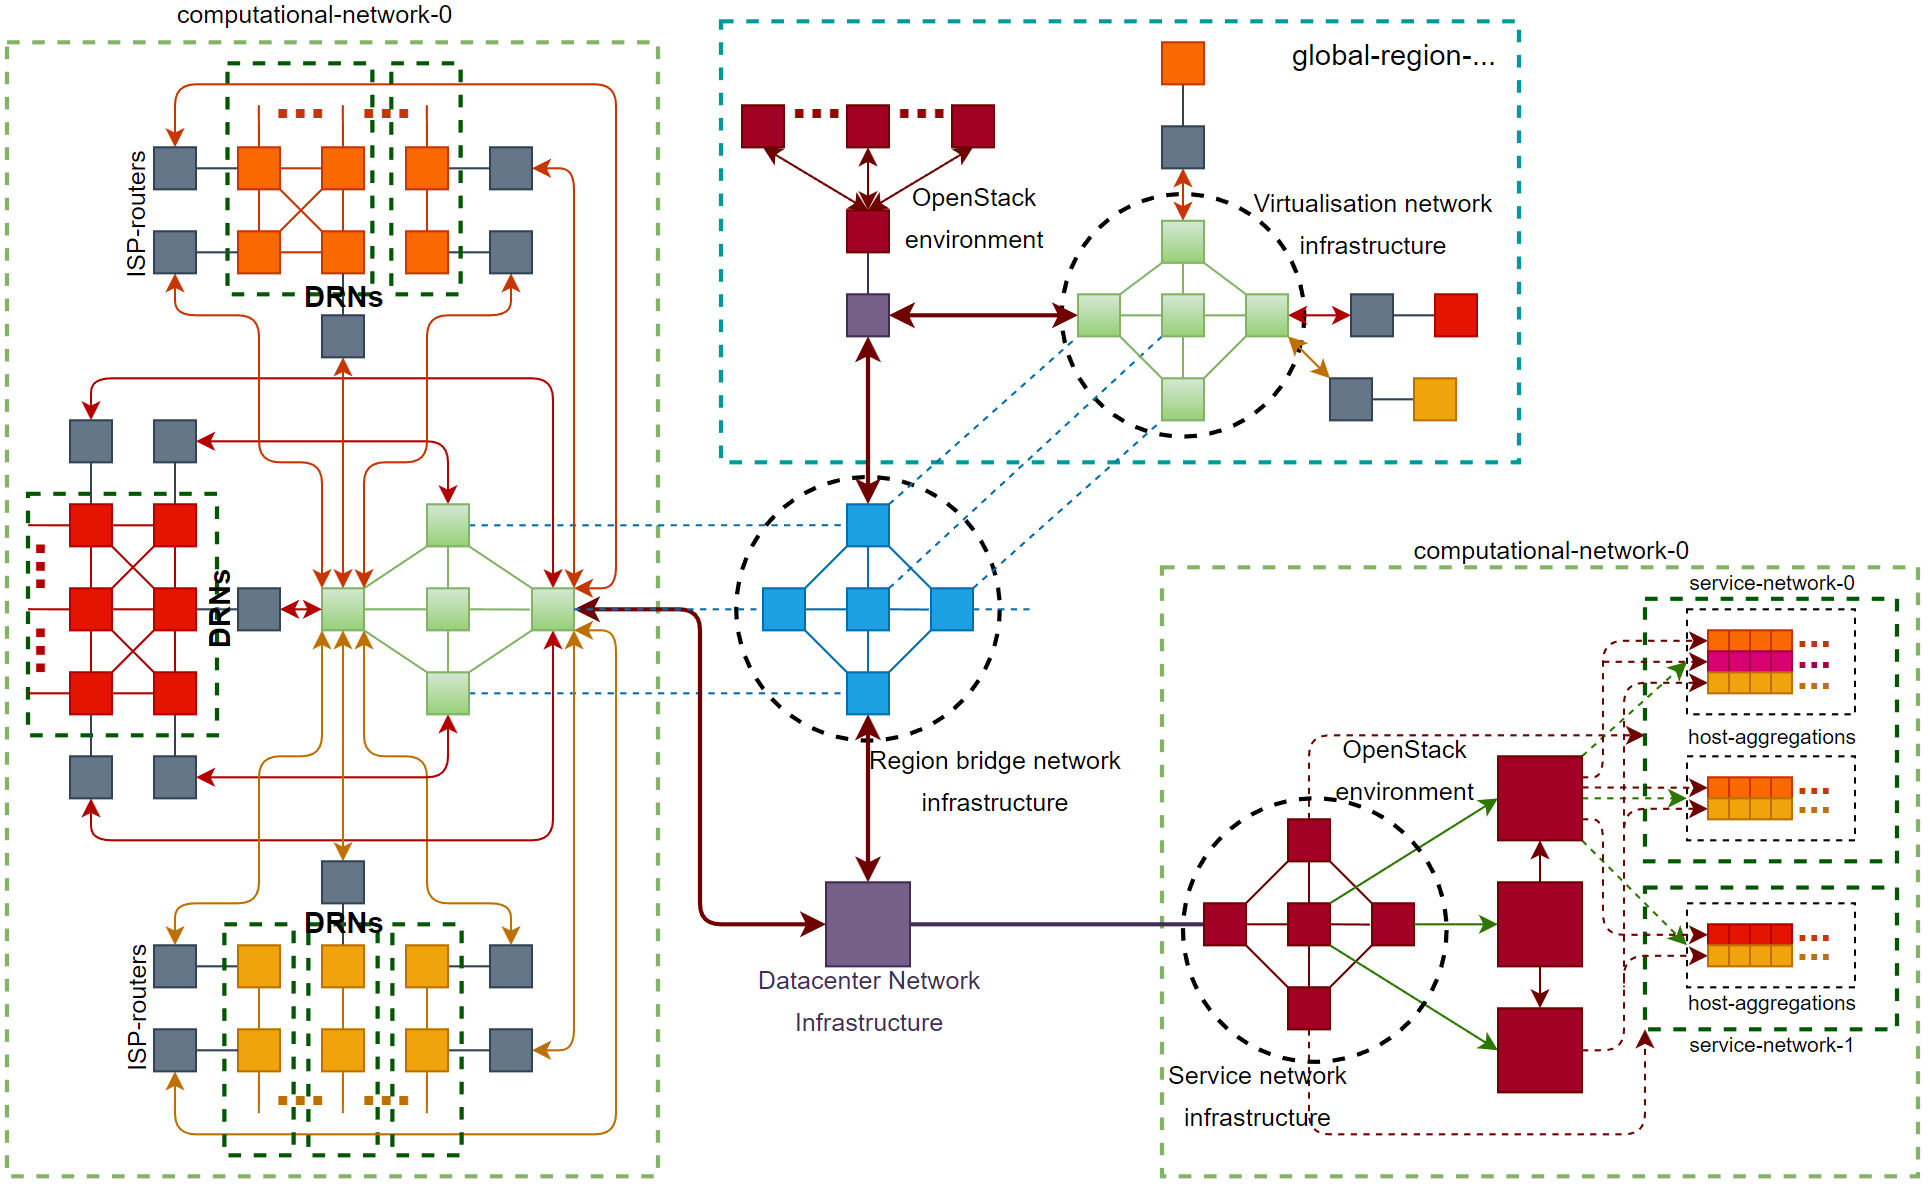
\includegraphics[height=9.5cm]{dvci-network-overview}
\end{center}
\begin{center}
	Figure 7: High-level overview of the DVCI Network approaches.
\end{center}

The fundamental idea here is to establish communication in the Logos network through an efficient low-latency network structure (external network service provider) with specific (Logos network) Software Defined Networks (SDNs). (What is Software-Defined Networking (SDN)? \cite{VMwareDoc-sdn})
These SDNs will be defined on the blockchain in order to "bring" the network sector onto the blockchain.
Since very low response times are not required for the Logos ecosystem and the network infrastructure is supported by SDNs, neither a very expensive nor a highly advanced network infrastructures (low-latency network structure) should be necessary.
\newline

% COMPUTATIONAL NETWORK
\textbf{Computational Network:}
These should be the main networks in a DVCI network environment.  
A low-latency software-defined network (computational network) should enable internal networking in a DVCI.  
Virtualization of physical hardware only makes sense and will function with optimum performance if the internal communication (DRNs with the dedicated root servers) runs with adequate latency times.
\newline

% SERVICE NETWORK
\textbf{Service Network:}
These networks are to be provided by the OpenStack environment for the Logos ecosystem services. 
Service networks are basically virtual networks that are provided by the OpenStack Network Nodes (neutron service). 
The intention is to separate services that run in different service environments (one or a set of host aggregates) across the computational network into separate service networks and make them efficiently accessible from the external world.
\newline

% REGION BRIDGE NETWORK
\textbf{Region Bridge Network:}
Region bridge networks (RBNs) are a concept in which services from one global region can access resources from another global region.
The basic idea behind RBNs comes from the so-called Gaming Private Networks (GPN), which optimize connection stability between a player and the game's servers. 
This is achieved by routing network packets on an optimized path between the user and the game servers.
This approach should make it possible to efficiently route and distribute DVCI resources on a global level.
\newline

All three of the network groups should be provided as SDNs at individual levels. 
Efficient ( Sufficiently efficient) network routes need to be provided by external Network Service Providers (NSPs) (for compute and region-bridge). 
This hardware network node infrastructure (provided via NSPs) should be optimized with the principle of SDNs specifically for the Logos network and thus reduce the overall cost of the NSP route nodes.  

It is important to notice, that this is a concept and only with the provision of the PoC the final proof can take place.
The detailed architecture and how the provision of such networks will be realized as well as their integration into the Logos network will be provided via the PoC in collaboration with external network experts.

% CONFIGURATION MANAGEMENT APPROACH
\subsubsection{Configuration and operation management approach}
The Logos network should be built as an automated or autonomous network. 
This can be achieved by using several existing technologies (Ansible, Terraform, ...), approaches and principles (GitOps, IaC CI/CD, ...). 

Infrastructure as Code (IaC) \cite{Wikipedia-iac} is an approach at managing and provisioning IT infrastructure resources through the use of declarative or imperative definitions.
The basic idea behind IaC is to treat the infrastructure in the same way as an application code, resulting in more efficient and consistent management of resources.

In a declarative approach (Terraform \cite{HashiDoc}), the infrastructure is described, as it should look, without explicitly specifying how it should be created. 
The desired state is specified and the IaC tool ensures that the infrastructure corresponds to this state.
In an imperative approach (Ansible \cite{AnsiDoc}), explicit instructions are given on how the infrastructure should be created and the IaC tool follows step-by-step instructions to achieve the desired configuration.

What makes the Logos network different in relation to IaC is that the code that will be executed by the IaC tools is on the blockchain in form of smart contracts.
Desired states or certain instructions of the infrastructure are defined on the blockchain.

The generation of transactions that trigger smart contracts is to be automated, which will be achieved by the Logos network gatekeeper component. 
Simply explained, the relevant network gatekeeper components should accept different instructions from the DVCI components, create transactions from them and execute them on the blockchain.

Another important strategy is the use of GitOps \cite{GitLabDoc} principles with CI/CD (continuous integration/continuous delivery) \cite{GitLabDoc-ci-cd} practices.
These practices aim to automate the development process, shorten development cycles, improve the quality of the code and create the possibility of fast and reliable deployments.

From version 1.0 we intend to hand over the sudo rights to the community, this approach (configuration and operation management of the Logos network) should enable transparency, controlled and easy access (for community authorized participants) and management of the network.

% FIGURE8
\begin{center}
	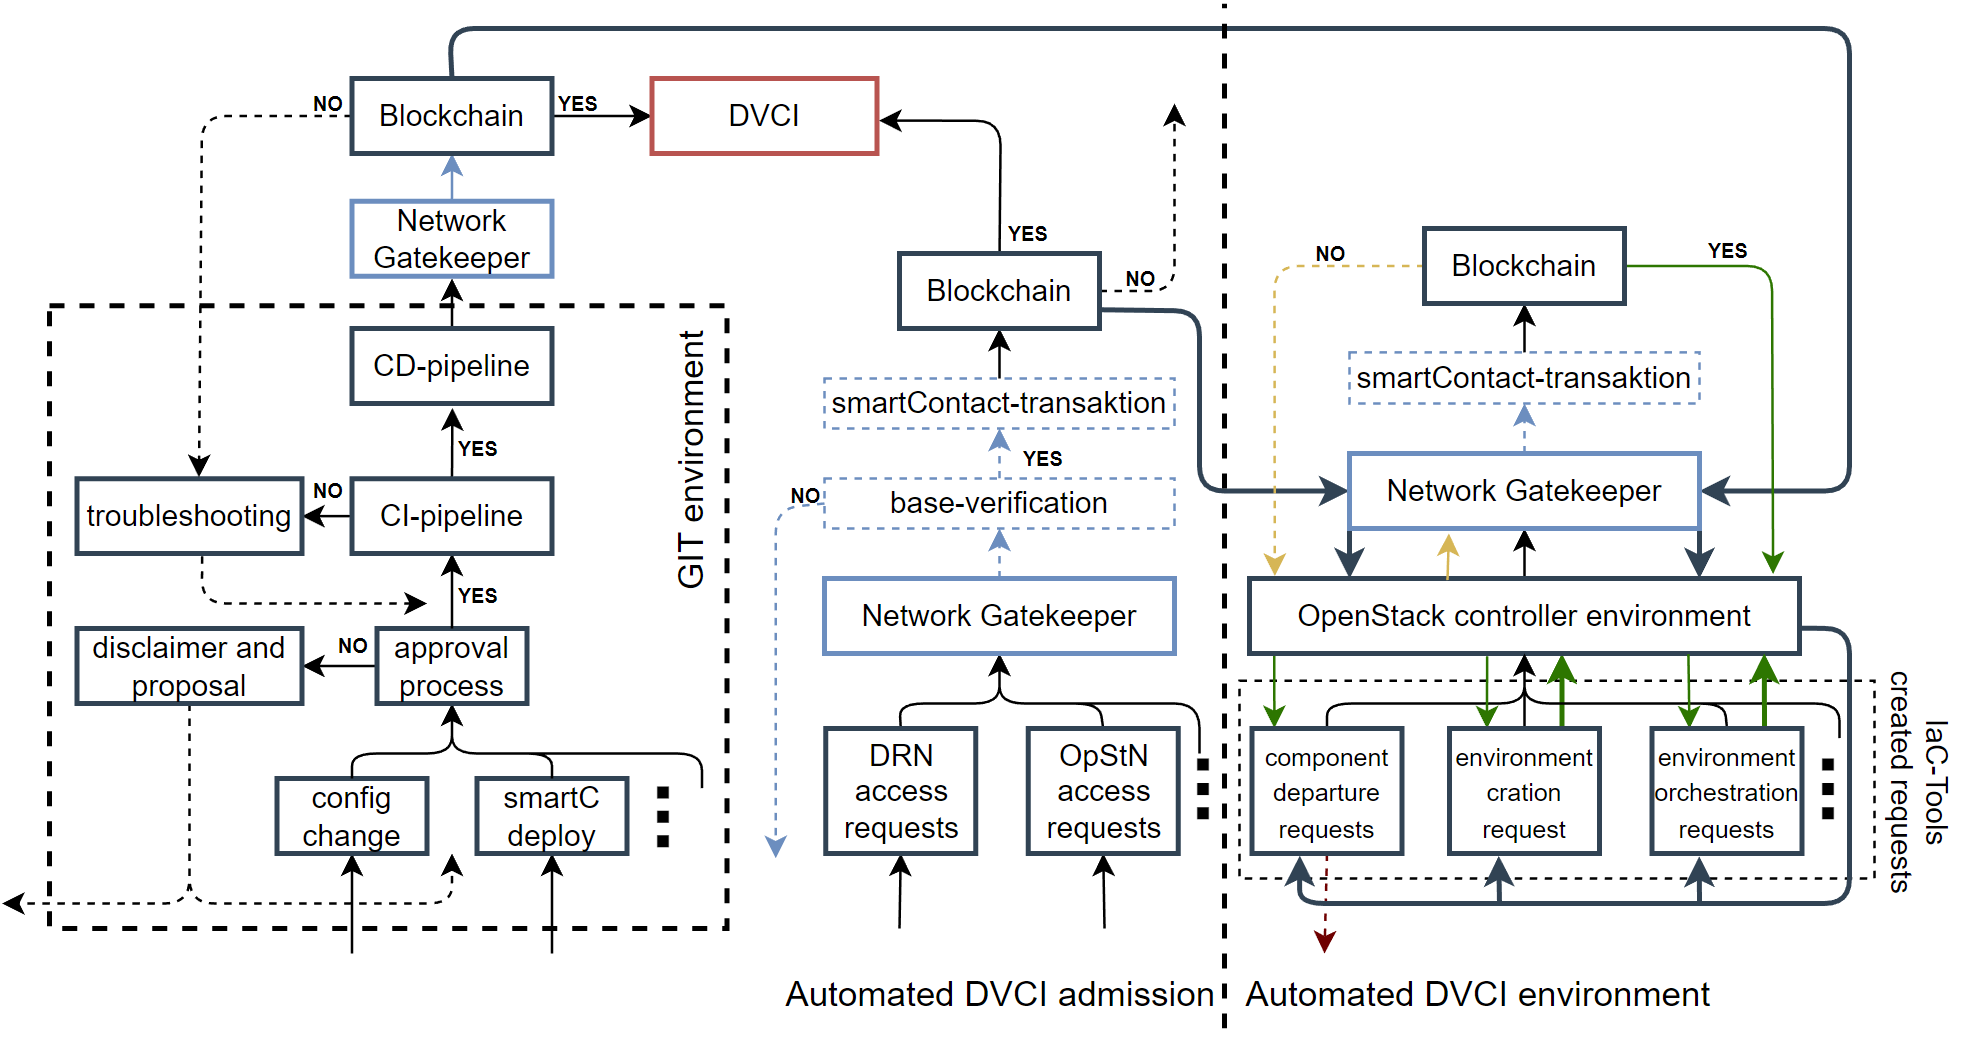
\includegraphics[height=8cm]{configuration-operation-management-approach}
\end{center}
\begin{center}
	Figure 8: High-level overview of the configuration, operation and management approaches of the Logos network.
\end{center}

% LOGOS CHAIN
\subsection{Logos Chain}
The Logos chain (blockchain component) is the basis for the Logos network. 
Until this point, although the DVCI is already a decentralized infrastructure it still functions in a conventional way (not web3).
Through the implementation of the DVCI into a blockchain, LogosLabs aims to create an additional security layer (sub0layer). 
This layer will secure the DVCI by the means of blockchain technology, thus providing a proper core infrastructure, web3 deserves.

The Logos chain should be developed as a layer-1 blockchain and be used to create and secure the sub0layer utilizing Smart Contract Logic, also being responsible for the implementation of certain functionalities (access to LN, payment options, transparency, ...) for web2 based services.

Smart contracts will be implemented in form of \textit{Smart Contract Logic}.
Smart contract logic should be an environment where different smart contracts are clustered by use case.
The Logos chain shall not be a public smart contract platform (Moonbeam, Astar, Phala Network, Cardano, ...).
An independent chain will have to be deployed to ensure specific smart contract implementations (type of SC, privacy features, SC configurations, ...). 
In order to create an efficient "system chain" all smart contracts on the Logos chain will have to be dedicated exclusively to the Logos network.
In principle, smart contracts on the Logos chain are not different from contracts on other chains, but the logic operating those contracts is.

The execution times of smart contracts do not play a major role in the overall network efficiency, since at this service layer participating nodes are not affected.
Should such a participating node get corrupted or become of a malicious nature, it will be subtracted from the DVCI (host aggregate or OpenStack environment).
Depending on how fast resources for a failed node (DRN) could be redirected back to its DVM, participating nodes would only have very short to no downtimes. 
Each host aggregation will have an additional 30\% backup buffer to further decrease possible downtimes (live VM-migration).
Smart contracts should only be triggered by the network gatekeeper, thus requiring a hybrid approach to confidentiality (public and private).

This hybrid approach, which allows for public and private elements to coexist, can limit access to the blockchain to only authorized accounts and certain access privileges (role-based access control principle).
Simply speaking, this approach would ensure a clear control over who has access to what and when.

Therefore combining the merits of both private networks and public infrastructures.
The Logos chain will be developed as a "parachain" (polkadot ecosystem) based on a substrate framework.
Polkadot and Substrate offer a highly advanced technological foundation for the development of decentralized applications and blockchain projects. 

% SUBSTRATE AND POLKADOT ECOSYSTEM
\subsubsection{Substrate and Polkadot ecosystem}
Substrate is an open-source framework developed by Parity Technologies, that enables the creation of custom blockchain networks for the Web3 era.
Substrate provides a set of tools and libraries, that allow to design and implement blockchain protocols.
It is specifically designed to facilitate the development of blockchain networks, while offering high flexibility and customizability. 
For a better understanding of Substrate, consider \cite{SubstrateDoc}.

There is a close connection between Parity Technologies and the Web3 Foundation in connection with Substrate, as Substrate was developed by Parity Technologies and is often used in conjunction with 
Polkadot, which was initiated by the Web3 Foundation. 

Polkadot is a blockchain platform, the main goal of which is to operate an interoperable and scalable platform for the Web3.
The basic idea behind Polkadot is to create a network of interconnected blockchains that promote scalability, security and interoperability.
Polkadot, as a layer-0 blockchain, is designed to overcome fragmentation in the blockchain ecosystem by connecting different blockchains (layer-1 blockchains). 
It enables secure and scalable interaction between them and promotes the flexibility and upgradeability of the overall system.
Each parachain \cite{PolkadotDoc-parachain} (layer-1 blockchains) has its own specific rules and consensus mechanisms, independent of the relay chain, while it (relay chain) acts as a link to enable overall security and interaction between the parachains.

Apart from interoperability (no focus of Logos network) and the ability to communicate with other parachains, Polkadot offers a number of other benefits and features (shared security, scalability, upgradeability, heterogeneity, community-driven governance, ecosystem diversity, ...).
For a more comprehensive understanding of Polkadot, read the original whitepaper \cite{Polkadot-whitepaper}.

% FIGURE9
\begin{center}
	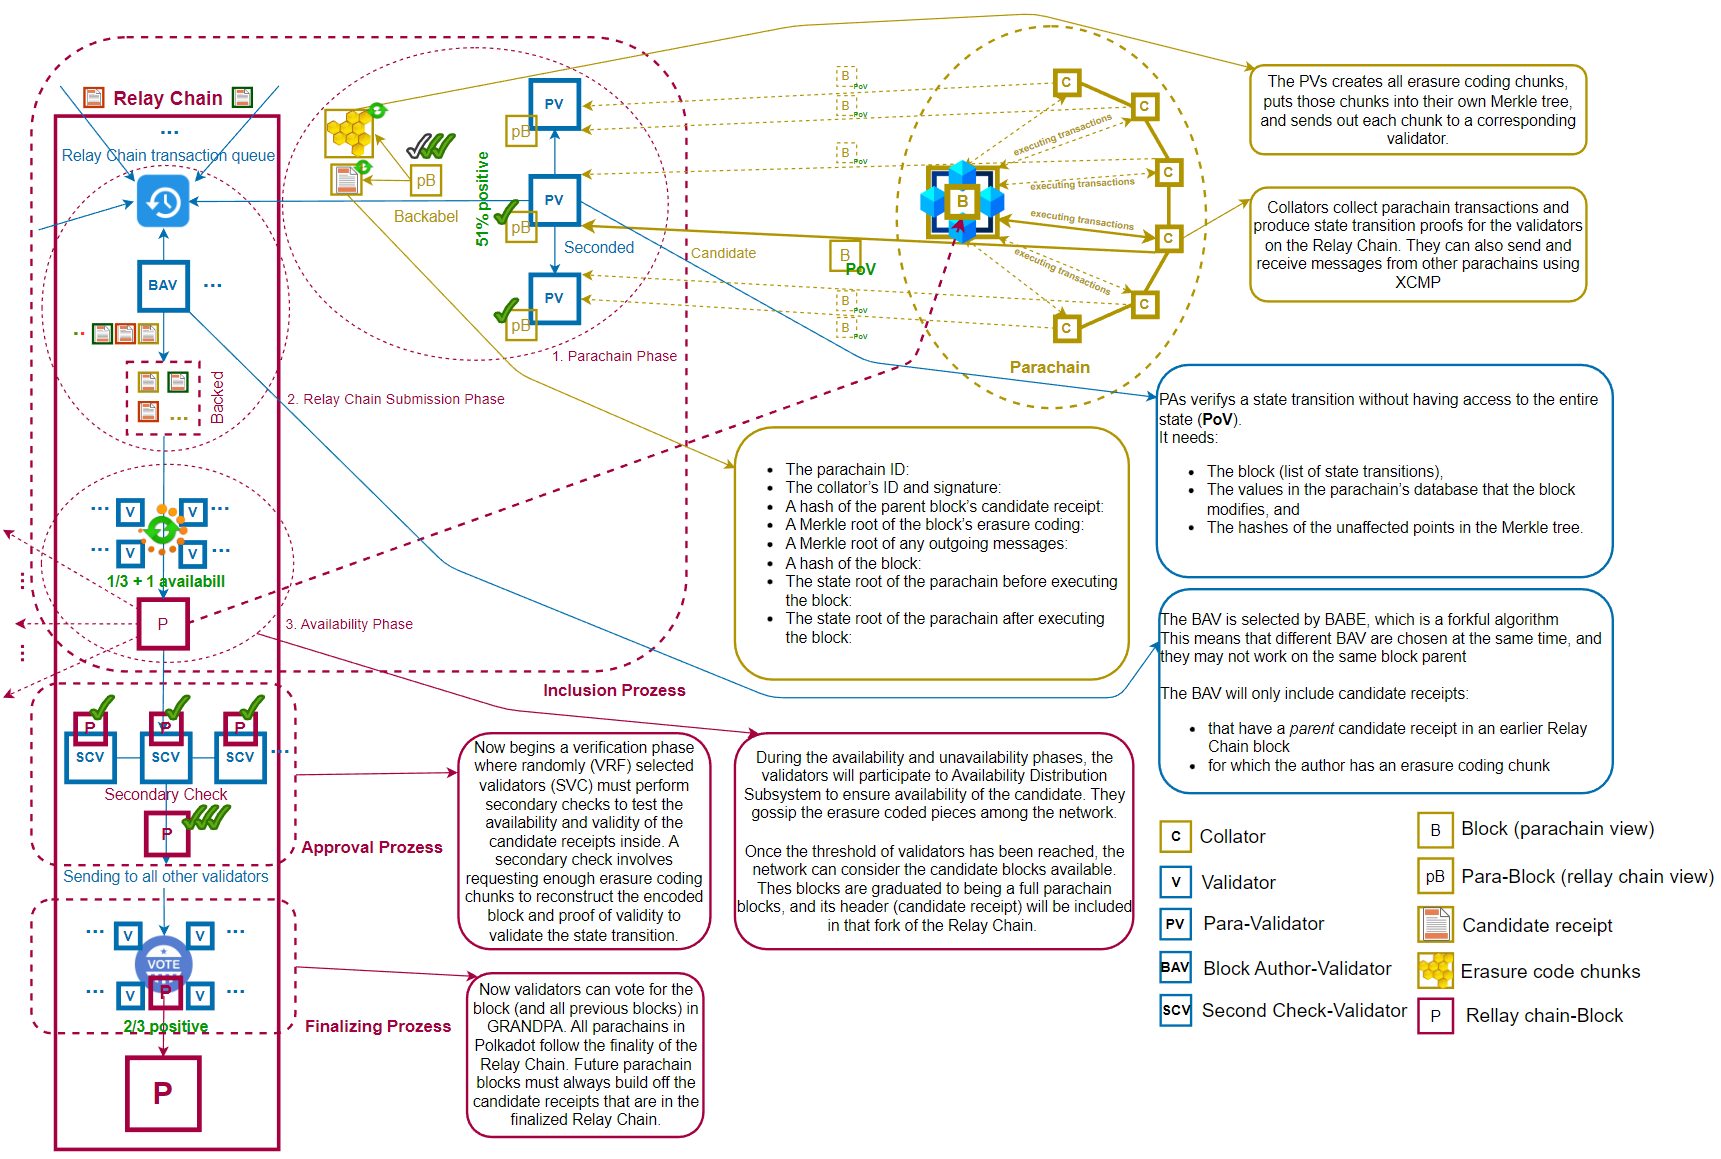
\includegraphics[height=10.2cm]{polkadot-tech-overview}
\end{center}
\begin{center}
	Figure 9: Overview of a Parachain Block Production in Polakdot 1.0. \cite{Parity-book-parachain}
	\newline
\end{center}

% ARCHITECTURE AND COMPONENTS
\subsubsection{Architecture and components}
The Web3 infrastructure is the technological basis for the development and provision of decentralized applications and the communication between them. 
It is a decentralized, interoperable and programmable infrastructure derived from blockchain and other distributed technologies.
A new web infrastructure is created by designating blockchain nodes to layer-0 and layer-1 blockchains.
From LogosLabs' perspective the decentralized approach is "the way to go" for the future. 

Blockchains in Substrate environments are defined by the runtime composition. 
Because the implementation of the DVCI will be carried out by smart contracts, the main focus of the runtime will have to be the provision of a infrastructural "Smart Contract Logic".

\textit{System-chains}, a term coined by polkadot \cite{PolkadotDoc-sys-parachain}, are chains containing the core protocols of the main system, and are exclusively tasked with network support (e.g. Asset Hub, Encointer, Bridge Hubs, ...). 
From a Logos Team's perspective, the resulting blockchain platform is a type of System-Chain. 
However system chains can only be viewed as such from the perspective of their respective networks. 
For this reason, polkadot will not categorize the logos-chain as a system parachain.

The blockchain "operates" or is "stored" on Substrate nodes that can have different roles and tasks therein.
Because we aim to become a parachain, the architecture has to be able to forward the proof of validity (PoV), created by the Logos chain (collator), to polkadot network participants (validator). 
Theoretically only collator nodes have to participate in candidate-block production, because they host both varieties of full-nodes (relay and parachain).
Not every type of node participates in block production/validation. 
Different types of substrate nodes exist (full node, archive node, light clients, validator node, collator node, boot nodes, ...) and will be responsible for different functionalities (transaction execution, transaction validation, interaction with the blockchain, ...).
These types of nodes (full, archive, light) augment the performance, security and accessibility of the main network participants (validator, collator).

% FIGURE10
\begin{center}
	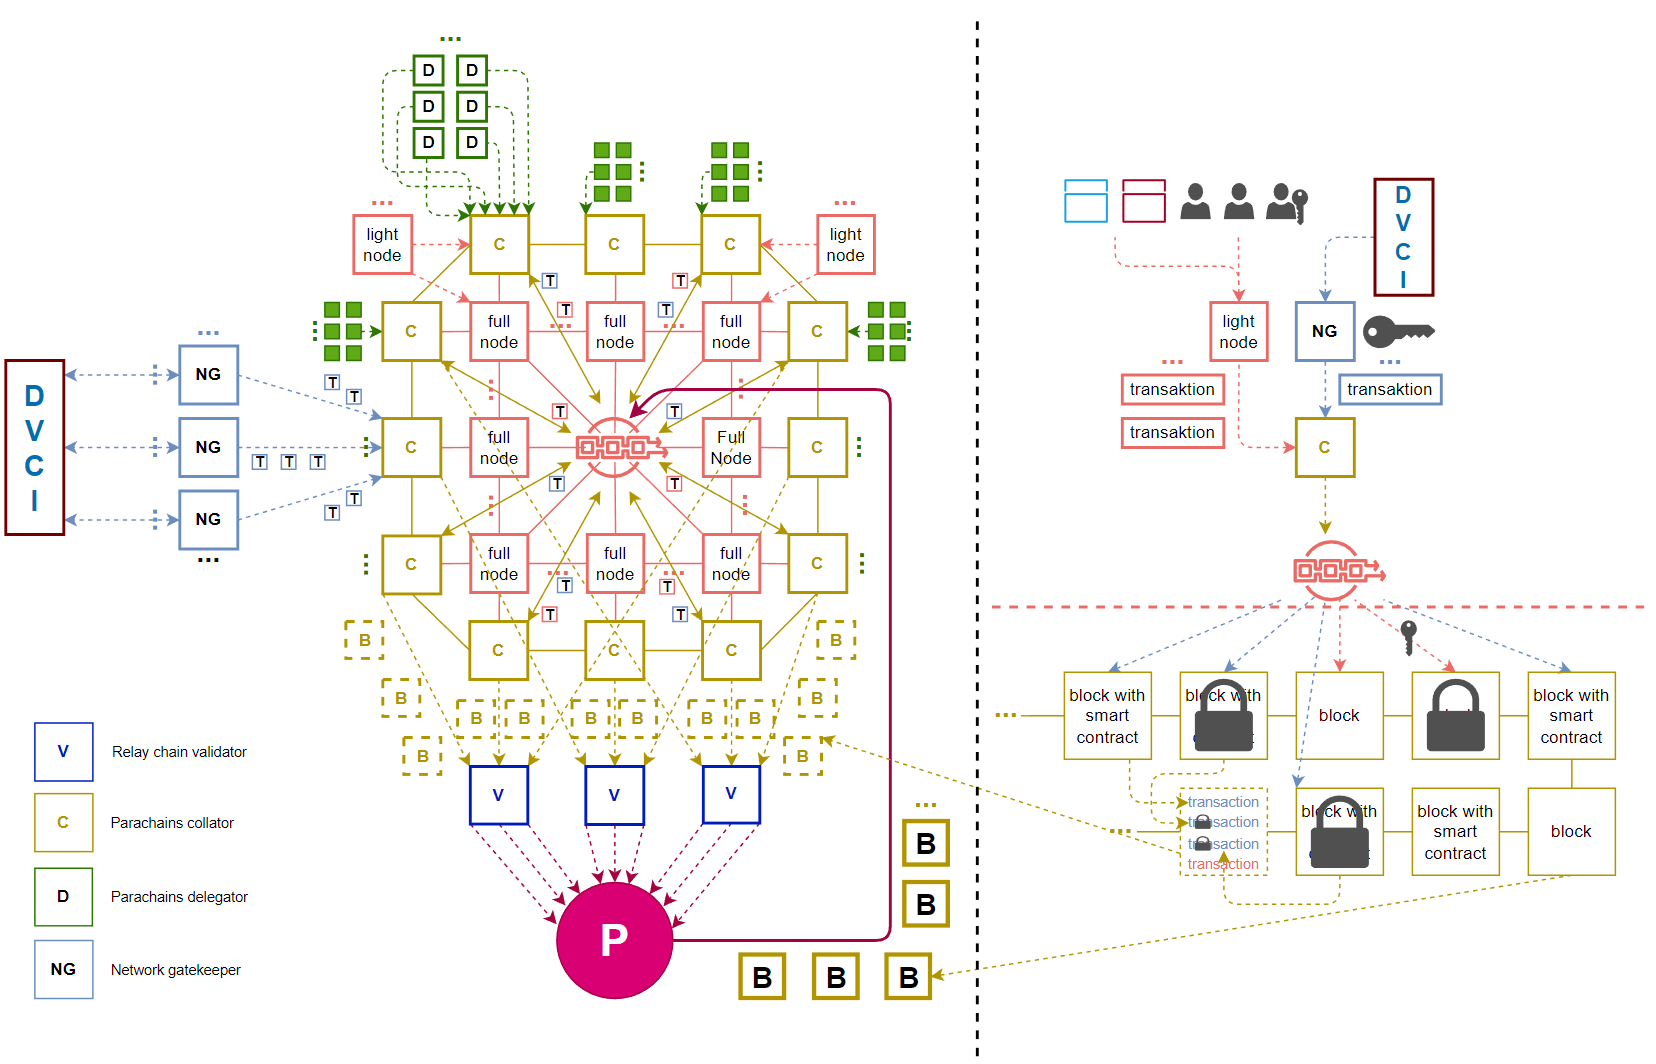
\includegraphics[height=10cm]{logos-chain}
\end{center}
\begin{center}
	Figure 10: High level overview of the Logos Chain and its components.
	\newline
\end{center}

% CLIENT AND RUNTIME
\textbf{Client and runtime:}
A Substrate Node basically consists of two main parts, the core client and the runtime.

The Substrate core client is the component that runs on a computer or server to interact with the Substrate network. 
It is a user interface that makes it possible to communicate with the blockchain, create transactions and retrieve information from the network.

Runtime is the heart of Substrate and embodies the logic that drives the blockchain.
The runtime determines whether transactions are valid or invalid and is responsible for processing changes to the blockchain state. 
External requests are forwarded to the runtime via the client, and the runtime is responsible for state transition functions and storing the resulting state.

The Substrate Runtime is designed for compilation in WebAssembly (Wasm) bytecode.
WebAssembly (Wasm) \cite{Webass} is a technology designed to compile code in a form that works efficiently, both on the web and on servers.
A significant benefit of using Wasm in Substrate is the ability to update the blockchain runtime without hard forks. 
As the runtime is available as a Wasm binary, it can be updated by the blockchain's governance system. 
This enables flexible and agile further development of the blockchain.
\newline

% SUBSTRATE LIBRARIES
\textbf{Substrate libraries:}
There are three types of libraries in Substrate that relate to the development of Substrate-based blockchains.
The Core Libraries, the FRAME Libraries and the Primitive Libraries.  

\begin{enumerate}[label=\textbullet]
	% CORE CLIENT LIBRARIES
	\item\textbf{Core client libraries:}
    These are libraries that enable a Substrate node to perform its network tasks, including consensus and block execution, as well as building the network layer, managing it and enabling communication between network participants and the transaction pool. 
	
	% FRAME LIBRARIES
	\item\textbf{FRAME libraries:} 
    The libraries that make it possible to create the runtime logic and to encode and decode the information transferred from the runtime.
    The FRAME libraries provide the infrastructure for the runtime.
    In addition to the infrastructure that is provided, the runtime can contain one or more "pallet" libraries.    
	
	% PRIMITIVE LIBRARIES
	\item\textbf{Primitive libraries:} 
	At the lowest level in the Substrate architecture, there are primitive libraries that provide control over the underlying operations and enable communication between the central outer client services and the runtime.	
\end{enumerate}
For detailed insights of the core-client, runtime and libraries, refer to \cite{SubstrateDoc-arch}

Composition and usage of FRAME, appropriate PALLETS as well the definition of the runtime-logic itself are subject to future research, hence the present shortage of specifics.
\newline

% NODES AND ROLES
\textbf{Nodes and Roles:}
Blockchain nodes are constantly synchronized and therefore provide a real-time overview of the blockchain-state.
The main focus of LogosLabs is to further secure the environment where these nodes are executed in (sub0layer).
Although Web3 provides a wide spectrum of security and development possibilities, the fact that participants are hosting nodes with big cloud providers, contradicts a true Web3 decentralized approach. 
In order to simplify the maintenance of security and integrity of the Logos chain, five types of nodes, able to interact with the network, will be utilized. 
Technically speaking are validators \cite{PolkadotDoc-validator} not bound to a specific blockchain and are thus excluded from further description. 

\begin{enumerate}[label=\textbullet]
	% COLLATOR NODE
	\item\textbf{Collator Node:} 
	Collators manage parachains by collating parachain transactions into parachain block candidates and creating proof-of-validity (PoV) for validation.
	Collators contain a full node for the relay chain and a full node for their specific parachain; this means that they keep all the necessary information to create new blocks and execute transactions, similar to what a miner does on PoW blockchains.
	For a deeper understanding of the collator role, review \cite{PolkadotDoc-collator}
	
	% FULL NODE 
	\item\textbf{Full Node:}
	Full nodes store blockchain data and typically participate in common blockchain operations, such as creating and validating blocks, receiving and verifying transactions, and providing data in response to user requests. 
	They support the network by ensuring consistency and reliability. 

    % ARCHIVE NODE
	\item\textbf{Archive Node:} 
	Archive nodes are similar to full nodes, with the difference that they store all past blocks with the complete status for each block. 
	Archive nodes are most commonly used by utilities such as block explorers, wallets, discussion forums and similar applications that require access to historical information.     
	
	% LIGHT CLIENT NODE
	\item\textbf{Light client node:} 
    Light Client Nodes enable interaction with a substrate network with minimal hardware requirements. They are not part of the blockchain or impact network operations. 
    They can be embedded in web-based applications, browser extensions, applications for mobile devices, ... .      
\end{enumerate}
For a better understanding of the base substrate nodes, consider \cite{SubstrateDoc-node}.

Every node can be configured individually. 
The access to nodes can be limited, nodes can be excluded from block production, communication restrictions can be imposed, etc.
The prospect of individual node configuration will play a major role in the implementation of the Logos network.

% SMART CONTRACT LOGIC
\subsubsection{Smart Contract Logic}
It is important to have a general understanding of the term smart contract \cite{SubstrateDoc-sc} before explaining the term Smart Contract Logic further.
Smart contracts are protocols that automatically, transparently and immutably execute contracts when predefined conditions are met. 
These contracts are written in code and are executed on a blockchain.
Smart contracts automatically execute actions as soon as the predefined conditions are met. 
There is no need for intervention once the code has been deployed.
Once deployed on a blockchain, the code of a smart contract cannot be changed without the consent of the network participants. 
This ensures the integrity and reliability of the contract.

The \textit{Smart Contract Logic (SCL)}, simply speaking is a comprehensive set of smart contracts, tasked with the execution of case specific instructions and measures.

Four types of contracts should be defined on the Logos chain:
\textit{configuration smart contract (CSC)}, \textit{operation smart contract (OSC)}, \textit{supply smart contract (SSC)} and \textit{web2to3 smart contract (W2t3SC)}. 
The first three smart contract types (configuration, operation and supply) are used to implement, secure and provision the DVCI, while the fourth type focuses on the provision of the "infrastructure" for web2 based services. 

The configuration smart contracts are intended to store the DVCI configurations in several central smart contracts. 
This makes it easier to manage and simplify the configuration data.
In a smart contract that manages configurations, each key-value pair represents a specific configuration or setting (important parameters or options for the system).

The OSCs perform certain operations or execution logic based on the configurations.
They will access CSCs in order to retrieve relevant configurations.

This type of structure allows a clear separation between the configuration and the operations elements, the key (key-value pair) plays a crucial role to identify the configurations.
Through this approach, we want to define the DVCI with one type of smart contract (configuration) and use the others (operations) to create this infrastructure and keep it operational.
Operations contracts can be used for each DVCI but the configuration smart contracts must be specific per DVCI.

The Substrate contracts pallet \cite{sub-contract-pallet}, as provided by default, focuses primarily on the creation and management of smart contracts within the Substrate framework. 
Its core functions include the development, deployment and execution of smart contracts, the management of storage and state of the contracts, interactions between different contracts and fee management for the execution of contracts. 

What the Substrate contracts pallet does not feature directly, however, are functions for use cases such as the separate storage and management of configuration data in standalone smart contracts.
If configurations are stored in separate smart contracts, they can be implemented modularly and reused by various other smart contracts. This enhances the reusability of code and configurations.
Separate smart contracts for configurations make it also possible to update configuration data independently of the main contract (operations smart contract). 
This can be useful if configurations need to be modified.

To implement a system for storing configurations in independent smart contracts, separate solutions must be developed within the contracts pallet. 
This may involve the creation of separate smart contracts for the management of configuration data or the development of special interfaces and protocols for communication and interaction between different contracts.

The supply contract type will be developed in such a way that the network gatekeeper and the W3bI (network provision service) can be defined and implemented on the chain. 
The technical implementation is not yet completely clarified, as there is the idea of splitting the supply contracts into configurations and operations elements. 
In principle, these will be contracts that support the DVCI operations.

The last type (web2to3) should be a conventional smart contract as it does not have to fulfill any special requirements.
This type of contract should enable the automated integration of web2 based services on the Logos network so that the resources of the network can be accessed.

In the smart contract logic, terms \textit{groups}, \textit{layers} and \textit{sections} should be differentiated.
In an infrastructure, there are various sectors such as network, security, computation, ..., which are divided here into so-called smart contract groups
The terms layer and section are very closely related. 
The DVCI is divided into different layers. 
In each of these layers, the DVCI is managed at a different level, so that, for example, the network is provided at different levels.
This creates these different sections (network-section-1, network-section-2, ..., compute-section-1, compute-section-2, ...) which are organized into different smart contracts.

The smart contracts will be developed with Rust \cite{rust-book} and the ink! Framework and compiled in Wasm bytcode so that they can be executed on the Substrate-based Logos chain. 
This is usually done with the Rust compiler, which is configured to compile Rust code in WebAssembly. 
The ink! Framework facilitates this process by providing the necessary tools and configurations.
For detailed insights of the ink! framework , refer to \cite{ink!articl}

The entire implementation of the smart contract logic will be provided with the PoC, as implementation solutions still need to be developed.   

% FIGURE11
\begin{center}
	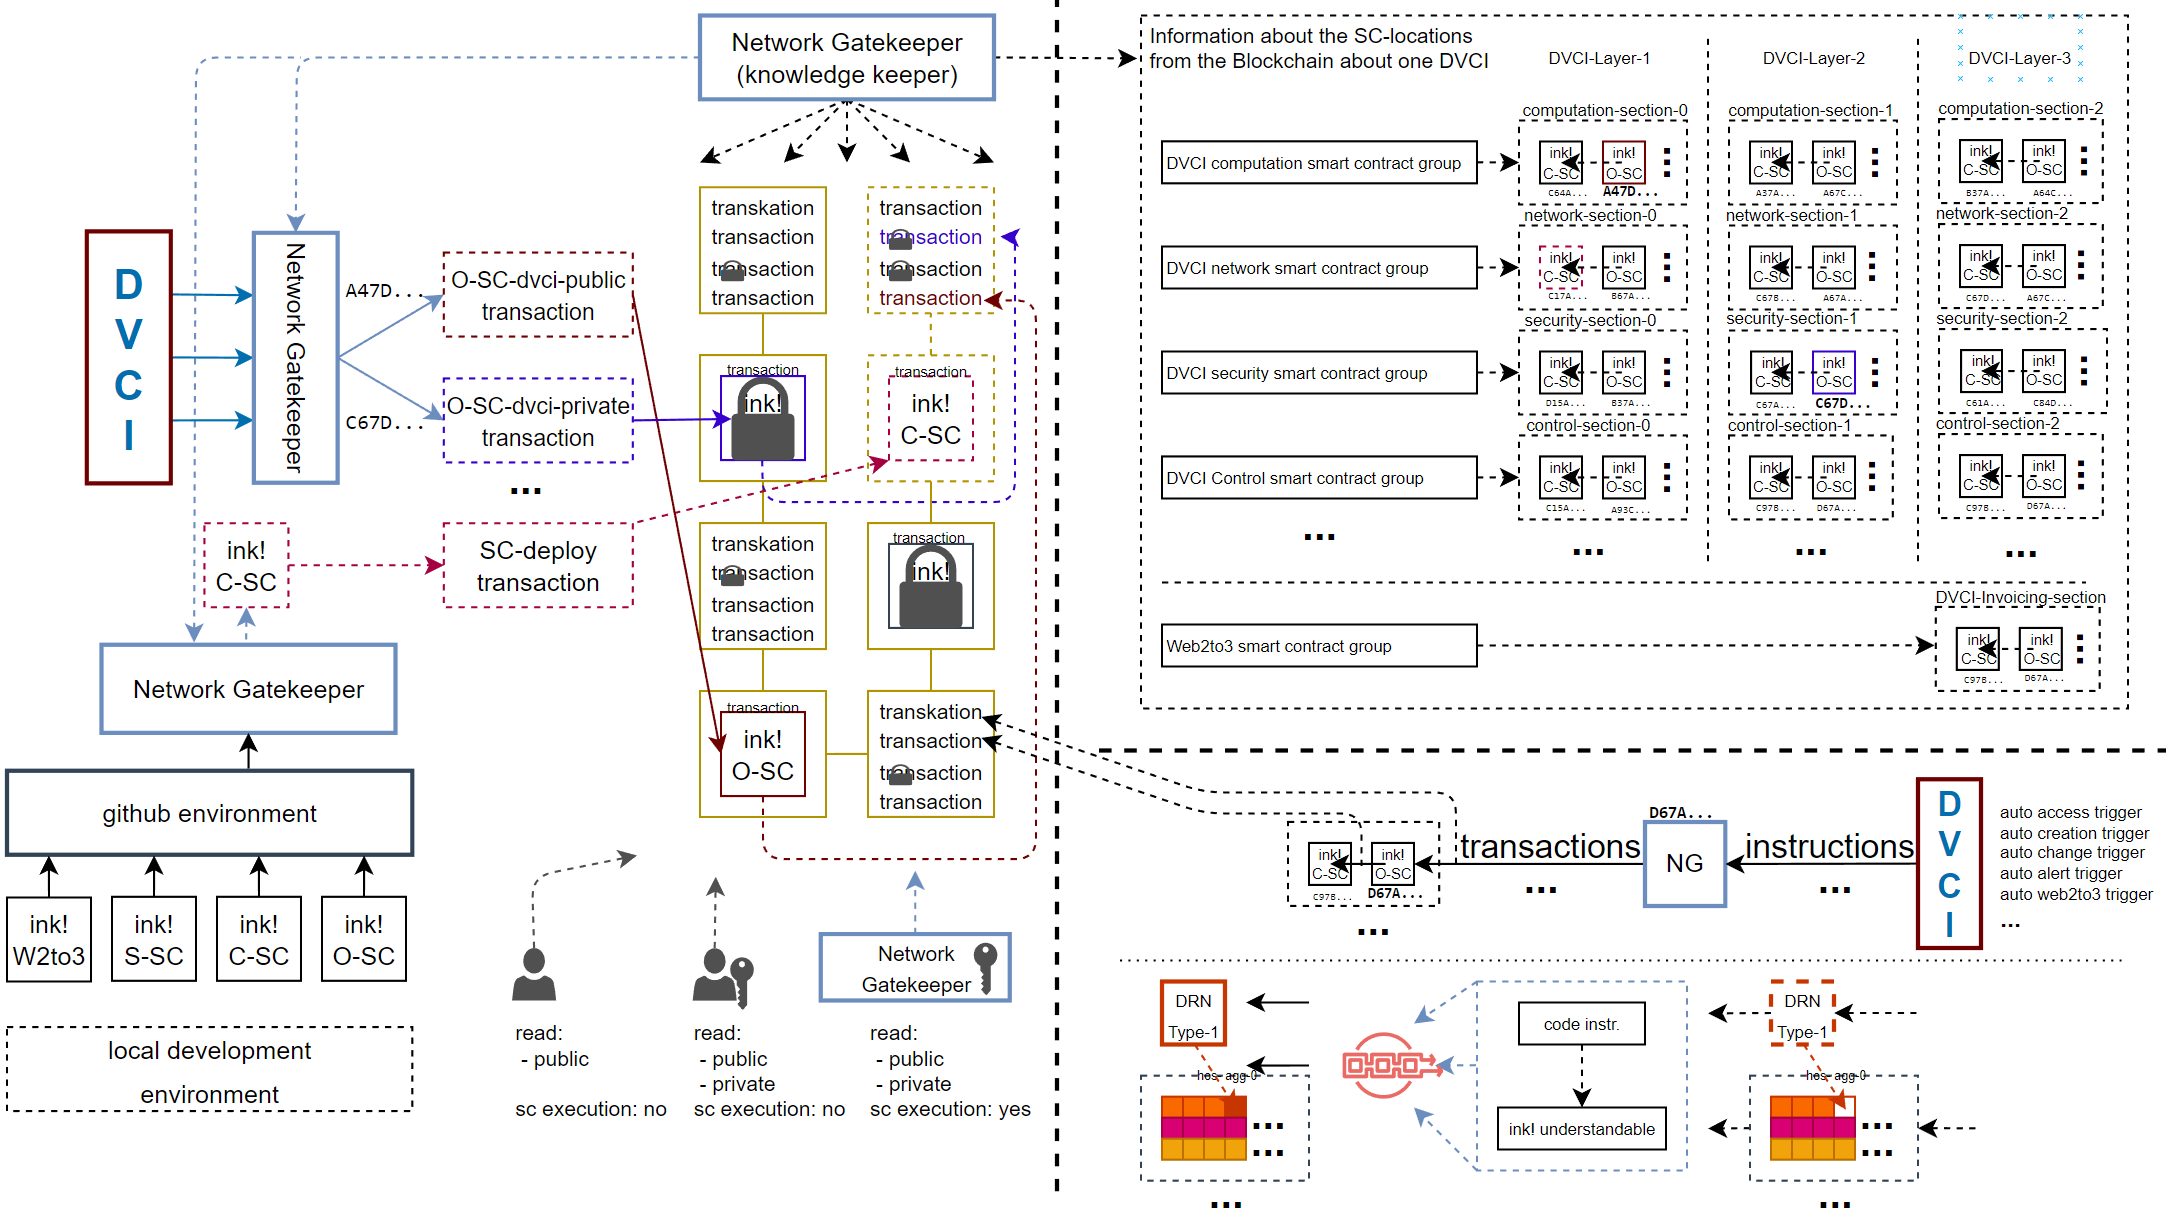
\includegraphics[height=8.6cm]{smart-contract-logic}
\end{center}
\begin{center}
	Figure 11: High level overview of the the smart contract logic implementation.
\end{center}

It is important to underline again that the approach is not the provision of an oracle, it is an attempt to operate the DVCI on-chain (smart contract execution time not relevant). 
From our perspective, the Logos network is the manifestation of what is defined on the blockchain.

% NETWORK GATEKEEPER
\subsection{Network Gatekeeper}
The network gatekeeper(NG), one of the most important components of the Logos network, will take on a multitude of tasks and will have to consist of multiple components. 
Communication between the DVCI and the blockchain will entirely depend on the NG. 
Another crucial duty of the NG will be the oversight of node behavior, in case of deviation of default node behavior, exclusion of affected participants and determination of the future procedure regarding those participants.
Simply speaking,this kind of \textit{middleware} (NG) will be used to define the DVCI and ensure the validity of its operations on the blockchain.  

The DVCI components will require different NG components to communicate with the blockchain.   
Not all of the DVCI components require all NG functionalities, which is why a distinction is made here between the \textit{Main NG} and the \textit{Client NG}.
The difference is that the Main NG includes additional components (\textit{DVCI validator}, \textit{Knowledge Keeper} and \textit{DVCI Book}). 
These components are required for the basic provisioning of the DVCI and are only installed on the OpenStack nodes since they are only required there.

The network gatekeeper (entirely) will be defined and executed on the Logos chain in the form of SSCs.
For example, when a component such as a DRN wants to participate in the network, the NG (client) that will enable its interaction with the blockchain will be first deployed on the DRN. 
The deployment of this NG on the DRN will be handled by blockchain operations (execution of SSCs) as well. 
This means that the client NG (client NG in this case) will only be deployed after the successful execution of the transaction and will be used to submit requests to the blockchain.

The reason for the development of the Network gatekeeper is primarily to enable such an automated infrastructure.
If you look at the CNCF (Cloud Native Computing Foundation) landscape \cite{cncf-land}, you realize how quick the development (technologically) in the cloud-native environment is progressing. 
The Web3 world can benefit from some of these technologies (currently benefits but to a certain level) and that is why we want to make it easier to implement such technologies with the NG, allowing them to be defined and used more simply "on-chain".
The network gatekeeper should enable automated communication of "cloud-native technologies" with the blockchain. 
This means that, for example, "native requests" (e.g. "kubeadm join ...") are understood by the blockchain via the gatekeeper and transactions can be triggered automatically to execute the request.

% FIGURE12
\begin{center}
	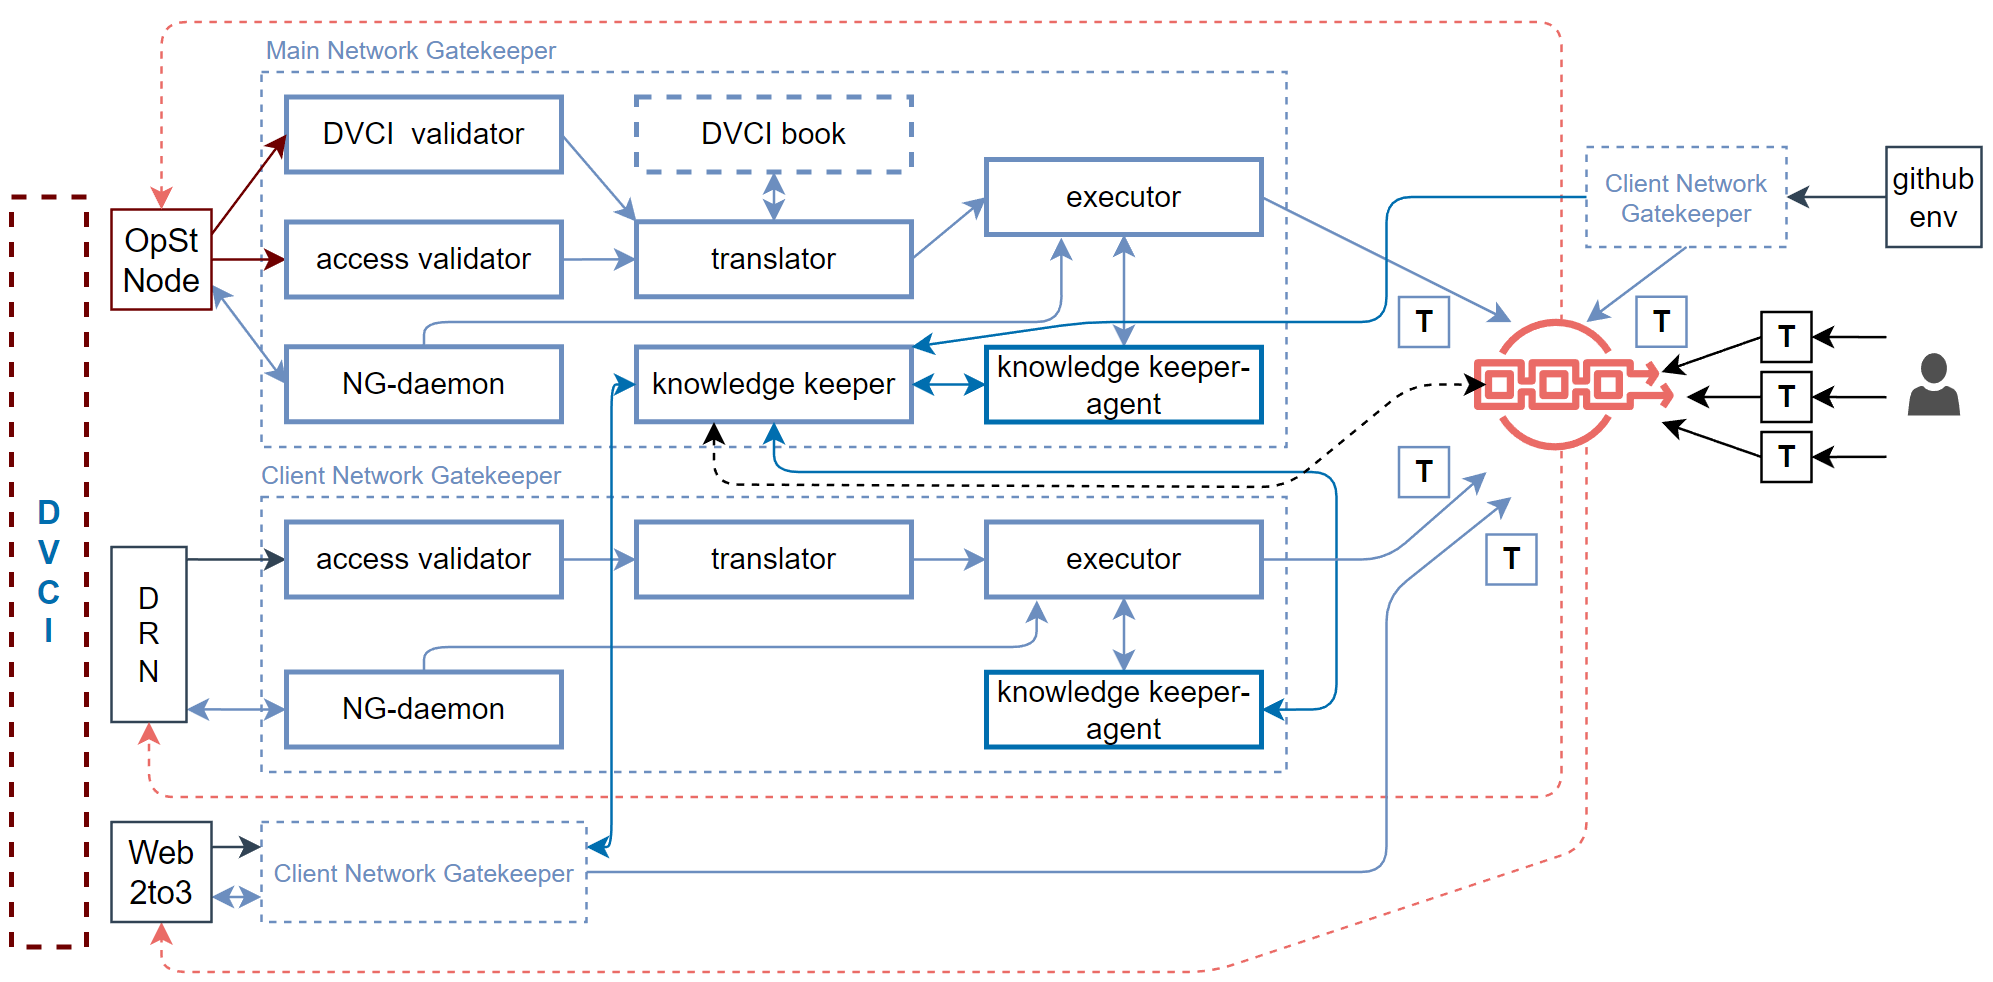
\includegraphics[height=7.5cm]{network-gatekeeper}
\end{center}
\begin{center}
	Figure 12: High level overview of the the Network Gatekeeper.
\end{center}

% ACCESS VALIDATOR
\textbf{Access validator:}
The \textit{Access Validator} will be responsible for the validation of incoming requests. 
Since not every random request should be forwarded to the blockchain, the \textit{AV} will have to perform a simple evaluation of the type of request and verify its compliance with prerequisites to trigger a transaction. 
In case a request is valid, it will be send to the "Translator".  
\newline

% DVCI VALIDATOR
\textbf{DVCI validator:}
The \textit{DVCI Validator} will process requests explicitly from the DVCI itself. 
Whereas the "AV" is appointed to DVCI-layer-1, \textit{DVCI-V} will be directed at layers 2 and 3.    
\newline

% TRANSLATOR
\textbf{Translator:}
The \textit{Translator} is a categorized set of data points with assigned key-values, created, sorted and validated by the "AV". 
The correct representation of these data points is necessary to produce a transaction, which will be the main task of the "TL". 
Simply speaking, the \textit{TL} will generate a request, in the required format (in form of a transaction) to trigger smart contracts, and forward it to the \textit{Executor}.   
\newline

% DVCI BOOK
\textbf{DVCI book:}
The \textit{DVCI Book} is an additional data-source for the \textit{TL}, a kind of vocabulary. 
\newline

% EXECUTOR
\textbf{Executor:}
The \textit{Executor} will deliver the request, with guidance from a \textit{Knowledge Keeper}, to the blockchain.   
\newline

% KNOWLEDGE KEEPER
\textbf{Knowledge keeper and the agent:}
The \textit{Knowledge Keeper} will contain data regarding the Smart Contract Logic. 
Furthermore the \textit{KK} will be tasked with the collection, organization and local storage of block chain data (SC location and metadata). 
In order for the Executor to receive the requested contract addresses (guidance) as fast as possible, an \textit{Agent} will be implemented to search the stored data.  
\newline

% NG-DAEMON
\textbf{Network gatekeeper daemon:}
The \textit{network gatekeeper daemon} will be the component responsible for security, thus playing a major role in the overall infrastructure. 
The \textit{NGd} will run on the host-OS of each component and ensure that the configurations "uploaded" to the node by the blockchain are intact and unchanged, otherwise excluding the node from the infrastructure under a zero-tolerance policy. 
\newline

The middleware (Network Getkeeper) will be developed as open source.
The focus of LogosLabs are "technologies" (OpenStack, Terraform, Ansible, ...) to be utilized for the Logos network.
Once the middleware is developed and functional, there is always the possibility to use the code to implement more solutions.  

% NETWORK REALIZATION
\subsection{Network realization}
At this point, all three key-components (DVCI, Logos chain and the network gatekeeper), comprising the Logos network, have been described in detail. 
Before deep-diving into the realization of the network and its role in the World Wide Web, the Logos network itself has to be distinguished from the services using it. 
Simply speaking, the Logos network will be an autonomous infrastructure that provides service-specific (Logos Ecosystem) computational/service environments, the services on the other hand will be "customers" (consumers of computational resources) of the Logos network.

As described earlier, the main intention of LogosLabs is to further secure and truly decentralize the Web3 infrastructure. 
This shall be accomplished by the "sub0layer" and the advantages Web3 presents over the conventional tech-sphere (Web2).

Figure 13 shows the entirety of the Logos Ecosystem in three stages.
The DVCI is fully defined on the blockchain(code) and will be supplied with enough physical hardware for its execution. 
The communication between the blockchain and physical hardware (via the network gatekeeper) is therefore required.    

% FIGURE13
\begin{center}
	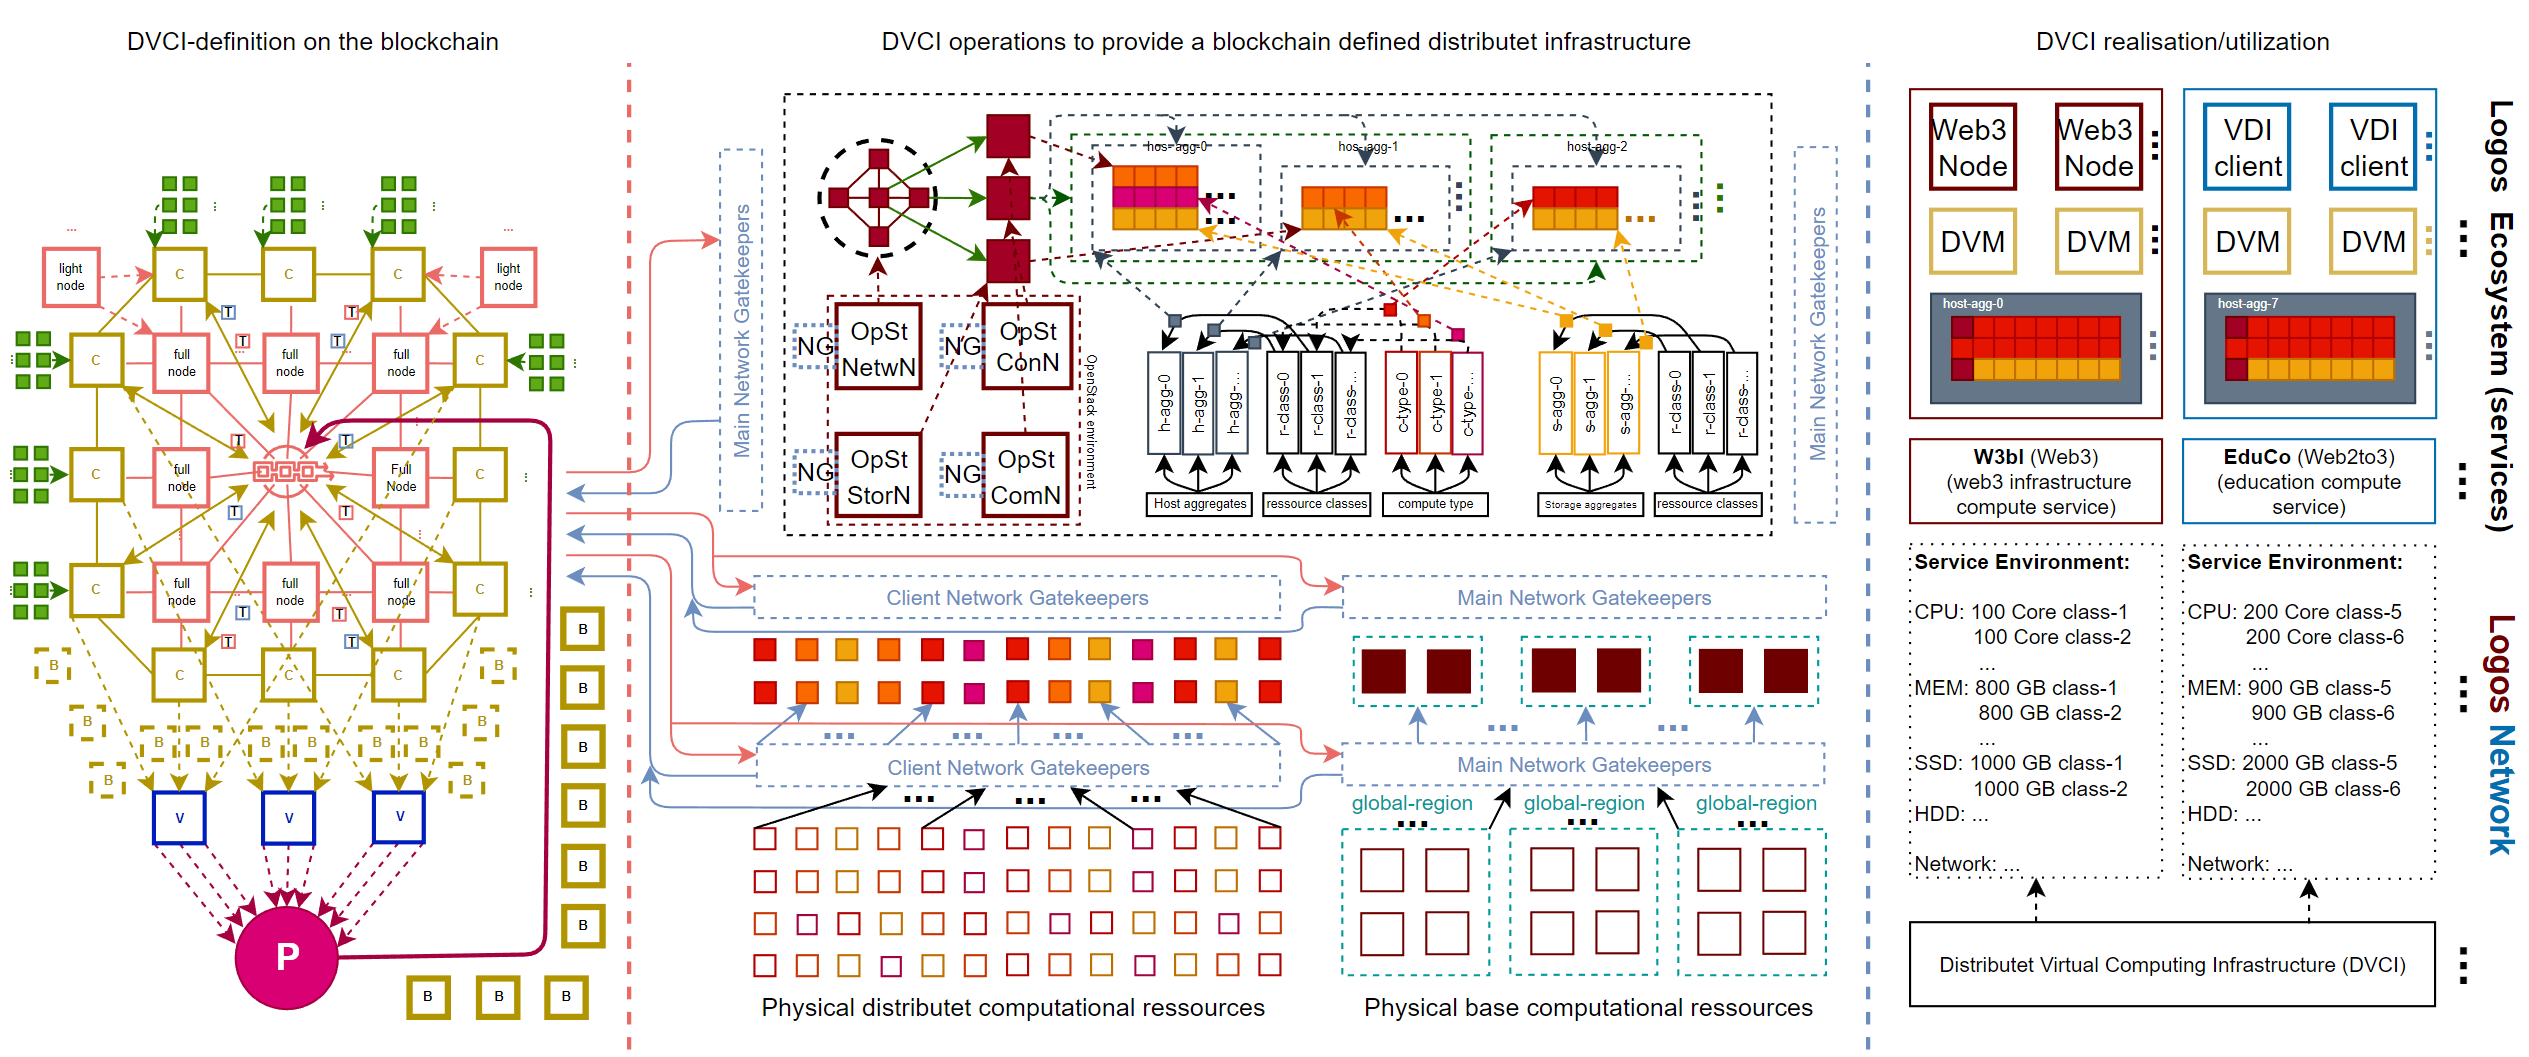
\includegraphics[height=6.4cm]{network-implementation}
\end{center}
\begin{center}
	Figure 13: General overview of how the Logos network will be utilized
\end{center}

Web2 services will be able to be developed and/or operated in the same manner as they are now. 
The only difference for those services would be a link to the blockchain, in order to ensure transparency in the compute-power billing process.
The network will not host Web2 services permanently.
Projects undergoing a migration to Web3 will be eligible for a temporary \textit{lease-time}, for the duration of said migration.
A Web3 service developed specifically for the advancement of Web3 infrastructures will be \textit{W3bI} (chapter 3.1).
The W3bI-service will simplify the deployment of Web3 services by providing the required blockchain nodes (Web3 infrastructure).

% FIGURE14
\begin{center}
	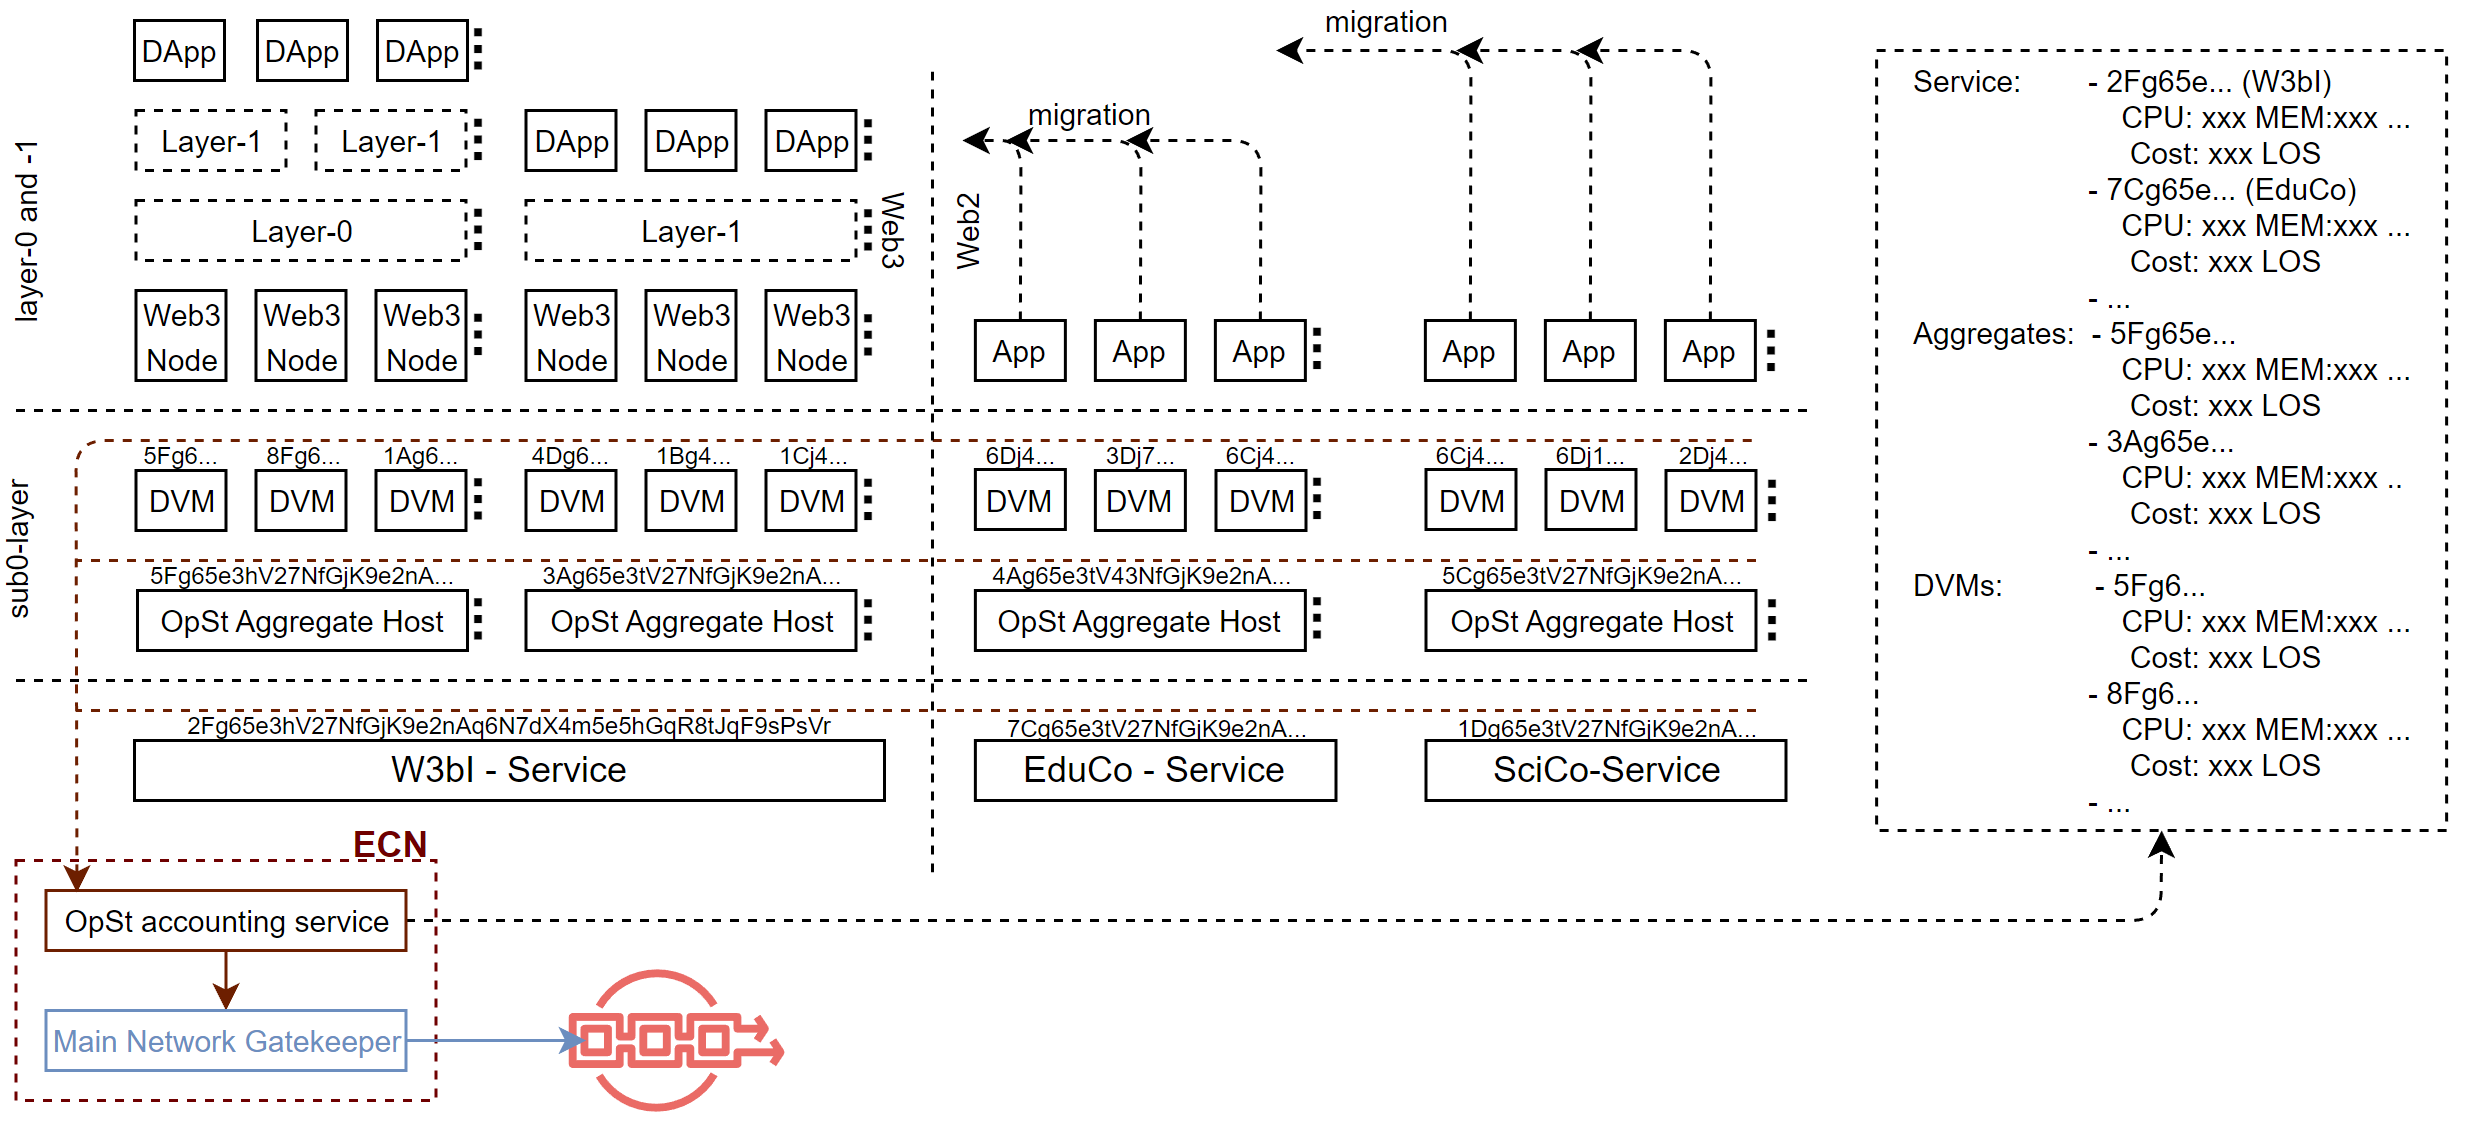
\includegraphics[height=6.9cm]{logos-network-services}
\end{center}
\begin{center}
	Figure 14: High level overview of the resource accounting implementation for Logos ecosystem services.
\end{center}

For the Logos network to be able to provide the required resources (service environments), the network must be reimbursed.
Such reimbursement should be carried out in the network's native currency.
The exact implementation will be defined once a governance system has been established. 

% SERVICE AND PROTOCOLS
\section{Services and protocols}
Services supported by the Logos Ecosystem will have access to computational resources provided by the DVCI (sub0layer), making the DVCI compatible with many Web2 and Web3 based cloud services.
This in turn will allow for the existence of a conventional cloud based infrastructure, provided by the community and secured by the blockchain.

The decision over the inclusion of a service into the network or a potential increase in compute power allocated to a service shall be, under the \textit{Logos network philosophy}, ruled on by the community.
The Logos network philosophy will be precisely defined by the first three services (W3bI, EduCo, SciCo).

The Logos network shall focus exclusively on these three fields; Decentralization, education and science.
Additional services could be implemented over time, provided they fit those fields.
The Logos ecosystem core service (W3bI), which will provide the fundamental computational infrastructure (for web3/blockchain infrastructure), shall be developed first. 
In addition to W3bI, two Web2 services shall be integrated (\textit{educational compute service - EduCo} and \textit{scientific compute service - SciCo}).   

The Logos network itself and the first three hosted services will be developed by LogosLabs. 
After the completed development (version 1.0) of the network, control over the network will be handed over to the community. 
The EduCo and SciCo services will continue to operate on the Logos network until the completion of the lease-time or as long as they fulfill the Logos network philosophy.

The same Logos network philosophy requirements applied to W3bI will be applied to all other services, but as W3bI is the core service of the ecosystem, the service will not have a conventional lease time as it is intended to facilitate the implementation of the Logos network itself into the World Wide Web.
The W3bI service will be developed and operated by LogosLabs in accordance with fair-price principles defined in the Logos network philosophy.
The approach of W3bI is to facilitate the provision of computational resources (Logos network resources) and not to be a profit oriented service.

The Logos network philosophy can be considered a kind of license.
This means that the specifications of the Logos network philosophy can be "enforced" by defined regulations in the SCL.

The development (to a certain degree) of ecosystem services during the actual Logos network development brings advantages.
The network is built to fulfill a specific purpose. This purpose always depends significantly on the requirements of the services it is supposed to serve.
Because of such an approach, the network should be fully ready for use at version 1.0 and appropriately tested, by already available services.

The main focus of this concept is to summarize and understand the idea behind the Logos network. 
However, since the services will play an important role during development, they are also fundamentally described in this paper. 
During the writing of the technical documentation (during the PoC), the EduCo and SciCo services will be treated as independent projects and will be described and explained in detail in their own technical documentations.

% W3BI
\subsection{W3bI}
The W3bI is the core service of the Logos network and of the ecosystem and will "host" blockchain nodes (layer-0 and layer-1 blockchain infrastructures).
The service will operate similarly to the current blockchain infrastructure providers, except that it will be defined on the blockchain itself and the core infrastructure used in the backend will be a full Web3 core infrastructure.
The W3bI service will be provided in a service environment made available by the Logos network.
An entire platform (Web3 IaaS) is to be developed and provided in this service environment.

For the provision of the W3bI service, the same implementation strategies will be used as for the Network Gatkeeper (supply smart contracts). 
Definition and execution on the blockchain to perform multiple functions.
W3bI will be defined on the same layer-1 blochain (Logos chain) as the Logos network itself, as it will handle the distribution of the Logos network resources and is therefore an important element of the ecosystem. 

This service should not be economically independent like EduCo or SciCo, since it is part of the network itself. 
Even if the service does not function completely autonomously and is maintained by LogosLabs, it must be regulated in order to comply with the "limited-profit" approach.
The "limited-profit" approach should become part of the Logos governance system.
This means that the provider (LogosLabs) of the W3bI service is obliged to comply with the pricing decided by the community in compliance with the Logos network philosophy.

Like the Logos network itself, W3bI will be part of the \textit{common-good} initiative to encourage and contribute to the development of Web3.

% CLOUD COMPUTING PLATFORM
\subsubsection{Cloud computing platform}
The type of platform (W3bI) that will be developed is generally referred to as a "Blockchain-as-a-Service" (BaaS) \cite{baas} platform. 
It is equivalent to other "as-a-Service" models in the cloud sector, such as Software-as-a-Service (SaaS), Platform-as-a-Service (PaaS) or Infrastructure-as-a-Service (IaaS) (IaaS/PaaS/SaaS definitions \cite{iaas-paas-saas}), but specifically focused on blockchain technologies.
This is a commonly used term that can be interpreted in many different ways.  
From the LogosLabs perspective, W3bI should be a \textit{Web3 IaaS platform/infrastructure}.

The W3bI platform is intended to offer a range of tools and services to simplify the process of deploying, maintaining and managing the Web3 infrastructure.
The functionalities of the blockchain (smart contracts, transaction processing, consensus mechanisms, ...) will not be provided by W3bI.   
The focus will be on providing the necessary hardware and network resources (through Logos network) required to operate these blockchain functions.
In short, the W3bI IaaS platform is a specialized form of cloud infrastructure that aims to simplify the setup and management of blockchain nodes, whereas the actual blockchain functionalities remain the responsibility of the developers of these blockchains.

The W3bI platform is generally intended to offer various options to further improve and facilitate the provision of the Web3 infrastructure.
Users will be able to set up and operate blockchain nodes without requiring technical knowledge. 
This platform will also offer tools and services for monitoring, maintaining and updating the nodes to ensure their continuous functionality and security. 
Another important aspect is scalability. 
Users will have the flexibility to increase or decrease the number of nodes as required.
These and other features make the W3bI platform an essential component for the efficient management and provisioning of the Web3 infrastructure (blockchain infrastructures).

% FIGURE15
\begin{center}
	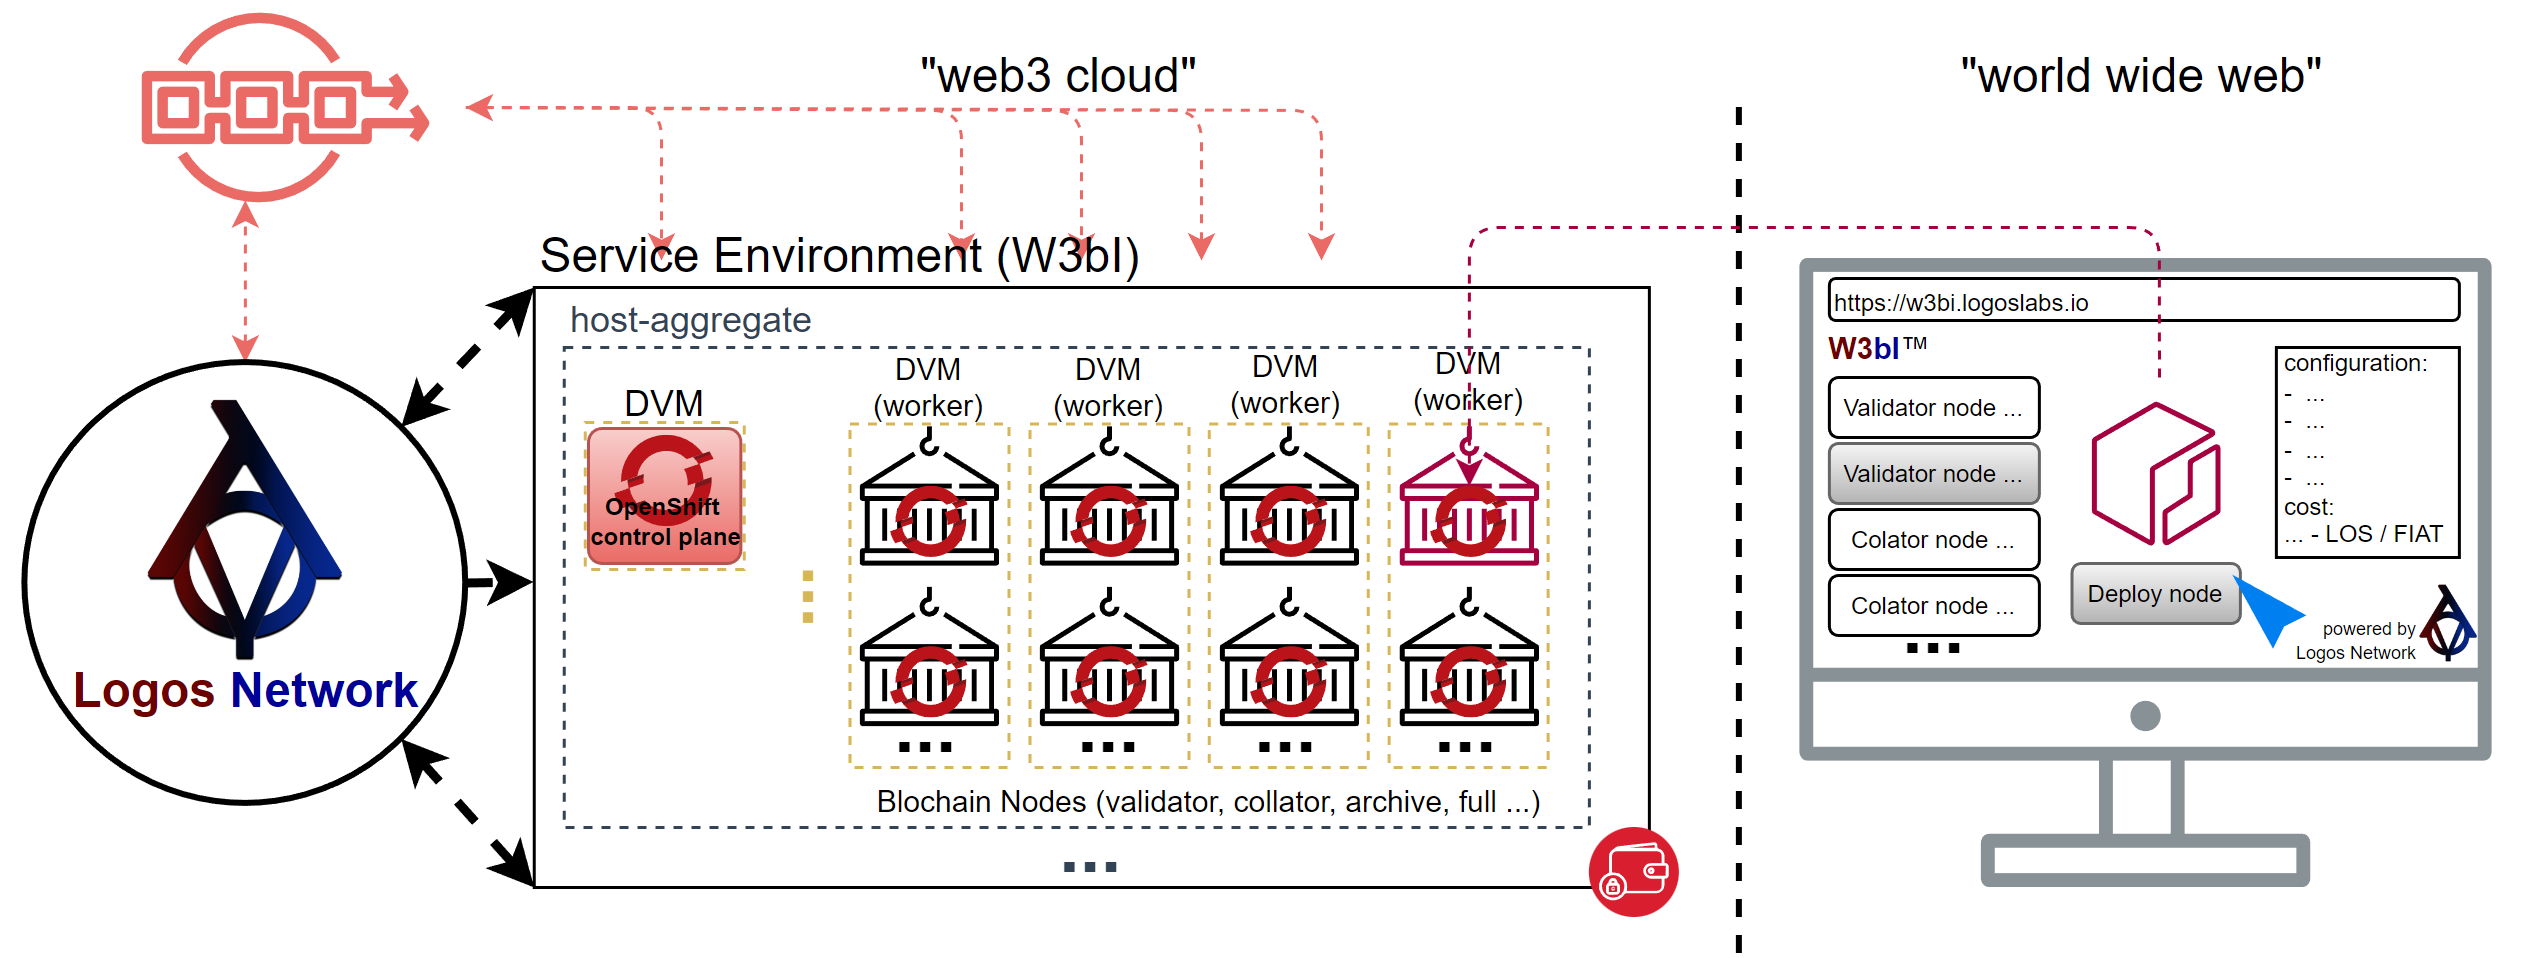
\includegraphics[height=5.5cm]{w3bi-overview}
\end{center}
\begin{center}
	Figure 15: High-level overview of the Web3 infratructure provider W3bI
\end{center}

This platform will be a Web3 based platform.
As described in the previous chapter, the service will be implemented on the blockchain in the form of SSCs. 
The important thing to note here is that the execution time of the SSCs on this layer has an impact on the service. 
For this reason, "off-chain" elements will be implemented here to make the platform more efficient. 

The terms "on-chain" and "off-chain" fundamentally refer to different types of data processing and storage.
"On-chain" refers to activities or transactions that take place directly on the blockchain.
"Off-chain", on the other hand, refers to activities that take place outside of the blockchain and are not stored on the blockchain.
 
Off-chain transactions are related to the blockchain, even if they take place outside the blockchain. 
They are part of the broader blockchain ecosystem and often interact in some form (complementary function, on-chain anchoring, trust anchor, ...) with on-chain data.
In practice, combinations of on-chain and off-chain solutions are often used to leverage the benefits of both approaches, especially in terms of performance, cost, scalability and privacy.

Detailed specifications of the architecture will be provided with the technical documentation.

% EDUCO
\subsection{EduCo}
A community based compute service for educational purposes was the main intent behind LogosLabs. 
However during the development of the concept we realized, that a sub0layer would also be advantageous for Web3 altogether, and further help counteract its increasing centralization.
For this reason, the main focus of LogosLabs shifted to the development of a sub0layer for all web3 infrastructures.

The reasoning behind EduCo is as follows: The amount of educational institutions (non IT), unable to upgrade existing pc-hardware or migrate to cloud services to offer students proper "present-day" tools, are progressively increasing.
The main reason for this increase is the extensive cost of physical hardware upgrades and cloud workspace services.
EduCo should solve this problem by being an affordable, community-driven, up-to-date alternative to existing cloud services. 
Relieving educational institutions of the need to upgrade physical hardware and providing them with a fairly-priced (community governance) payment model (\textit{pay-as-you-use}) \cite{WikipediaDoc-payu} for compute-units.
The connection of "user-workstations" to the network would be accomplished by the \textit{LogBox}, a simple yet efficient single-board device, capable of accessing the cloud workspace as well as operating a wallet to reimburse the network (providers).

\textit{The LogBox shall be the last piece of computational hardware, educational institutions (non-IT) will ever need.}  

% CLOUD WORKSPACE PLATFORM
\subsubsection{Cloud workspace platform}
A Cloud Workspace Platform (EduCo) will be a cloud-based solution that provides virtual work environments where users can access applications, data and services regardless of their physical location. 
This approach offers a range of features and benefits (flexibility and mobility, cost efficiency, scalability, maintenance and upgrades, easier compliance, centralized management, ...)
The platform will be designed to support productivity and flexibility, as well as the reduction of IT complexity (local IT infrastructure and maintenance). 

At its core, the platform will consist of a large number of servers and storage systems (DRNs) within host aggregates. (Service environment) 
These resources (within host aggregates) are divided into several efficient virtual servers (DVMs).
Such a solution allows different "tenants" to use the same host resources (host aggregates) while keeping their data and applications in an isolated and secure environment.

The applications and services that will be available on the EduCo platform will be web-based and will follow the software-as-a-service model, which means that users will be able to use the service via a browser-based solution or via the \textit{single board client} (chapter 2.2) without having to install anything locally.

A central element of a cloud workspace solution is identity and access management, which ensures that only authorized users can access the required resources. 
This should be achieved through technologies such as single sign-on and multi-factor authentication.

This type of platform will be possible with the support of RDPs and the implementation of VDI solutions.
\newline

% REMOTE DESKTOP PROTOCOLS
\textbf{Remote desktop protocols:}
Remote Desktop Protocols (RDPs) \cite{WikipediaDoc-rdp} are protocols (Microsoft's RDP, RFB (Remote FrameBuffer), SPICE (Simple Protocol for Independent Computing Environments), ...) that make it possible to access and control the graphical user interface (GUI) of a remote computer or server. 
This makes it possible to access resources and applications from a remote location as if you were sitting in front of the computer.
\newline

% VIRTUAL DESKTOP INFRASTRUCTURE
\textbf{Virtual desktop infrastructure:}
Virtual Desktop Infrastructure (VDI) \cite{VMwareDoc-vdi} (Apache Guacamole, oVirt, Virt-Manager, ...) enables desktop environments to be hosted centrally in a virtualized form and made available via the network. 
Essentially, the entire desktop environment is virtualized in a cloud environment and can be accessed via end devices such as PCs, laptops or thin clients.
\newline

The EduCo platform is intended to offer VDI solutions for educational institutions.
A thin client (single board client) will be provided for such institutions to connect to the EduCo service.  

The detailed specifications and the implementation itself should be provided in the PoC and with the technical documentation. 
There are several VDI/RDP solutions (Apache Guacamol/VNC-RFB, SPICE/SPICE, FreeRDP/OpenSource Microsoft's RPD) which should be evaluated before a decision is made which of the technologies or solutions is the most applicable to the EduCo service.  

The "platform provider" (EduCo) will be responsible for managing the entire platform, including maintenance, performing updates, backing up data and implementing disaster recovery plans.
Altogether, EduCo will provide a comprehensive, secure and efficient virtual working/teaching/learning solution that supports the modern way of education through flexibility, scalability and accessibility.

It is important to point out that a Web2 solution has been described in this section.
After the platform is implemented as a web2to3 service on the network, the focus will be set on the migration to a layer-1 blockchain. 
The reason for this interim step is to develop integration solutions for future web2 services that will use the network during their migration. 

% FIGURE16
\begin{center}
	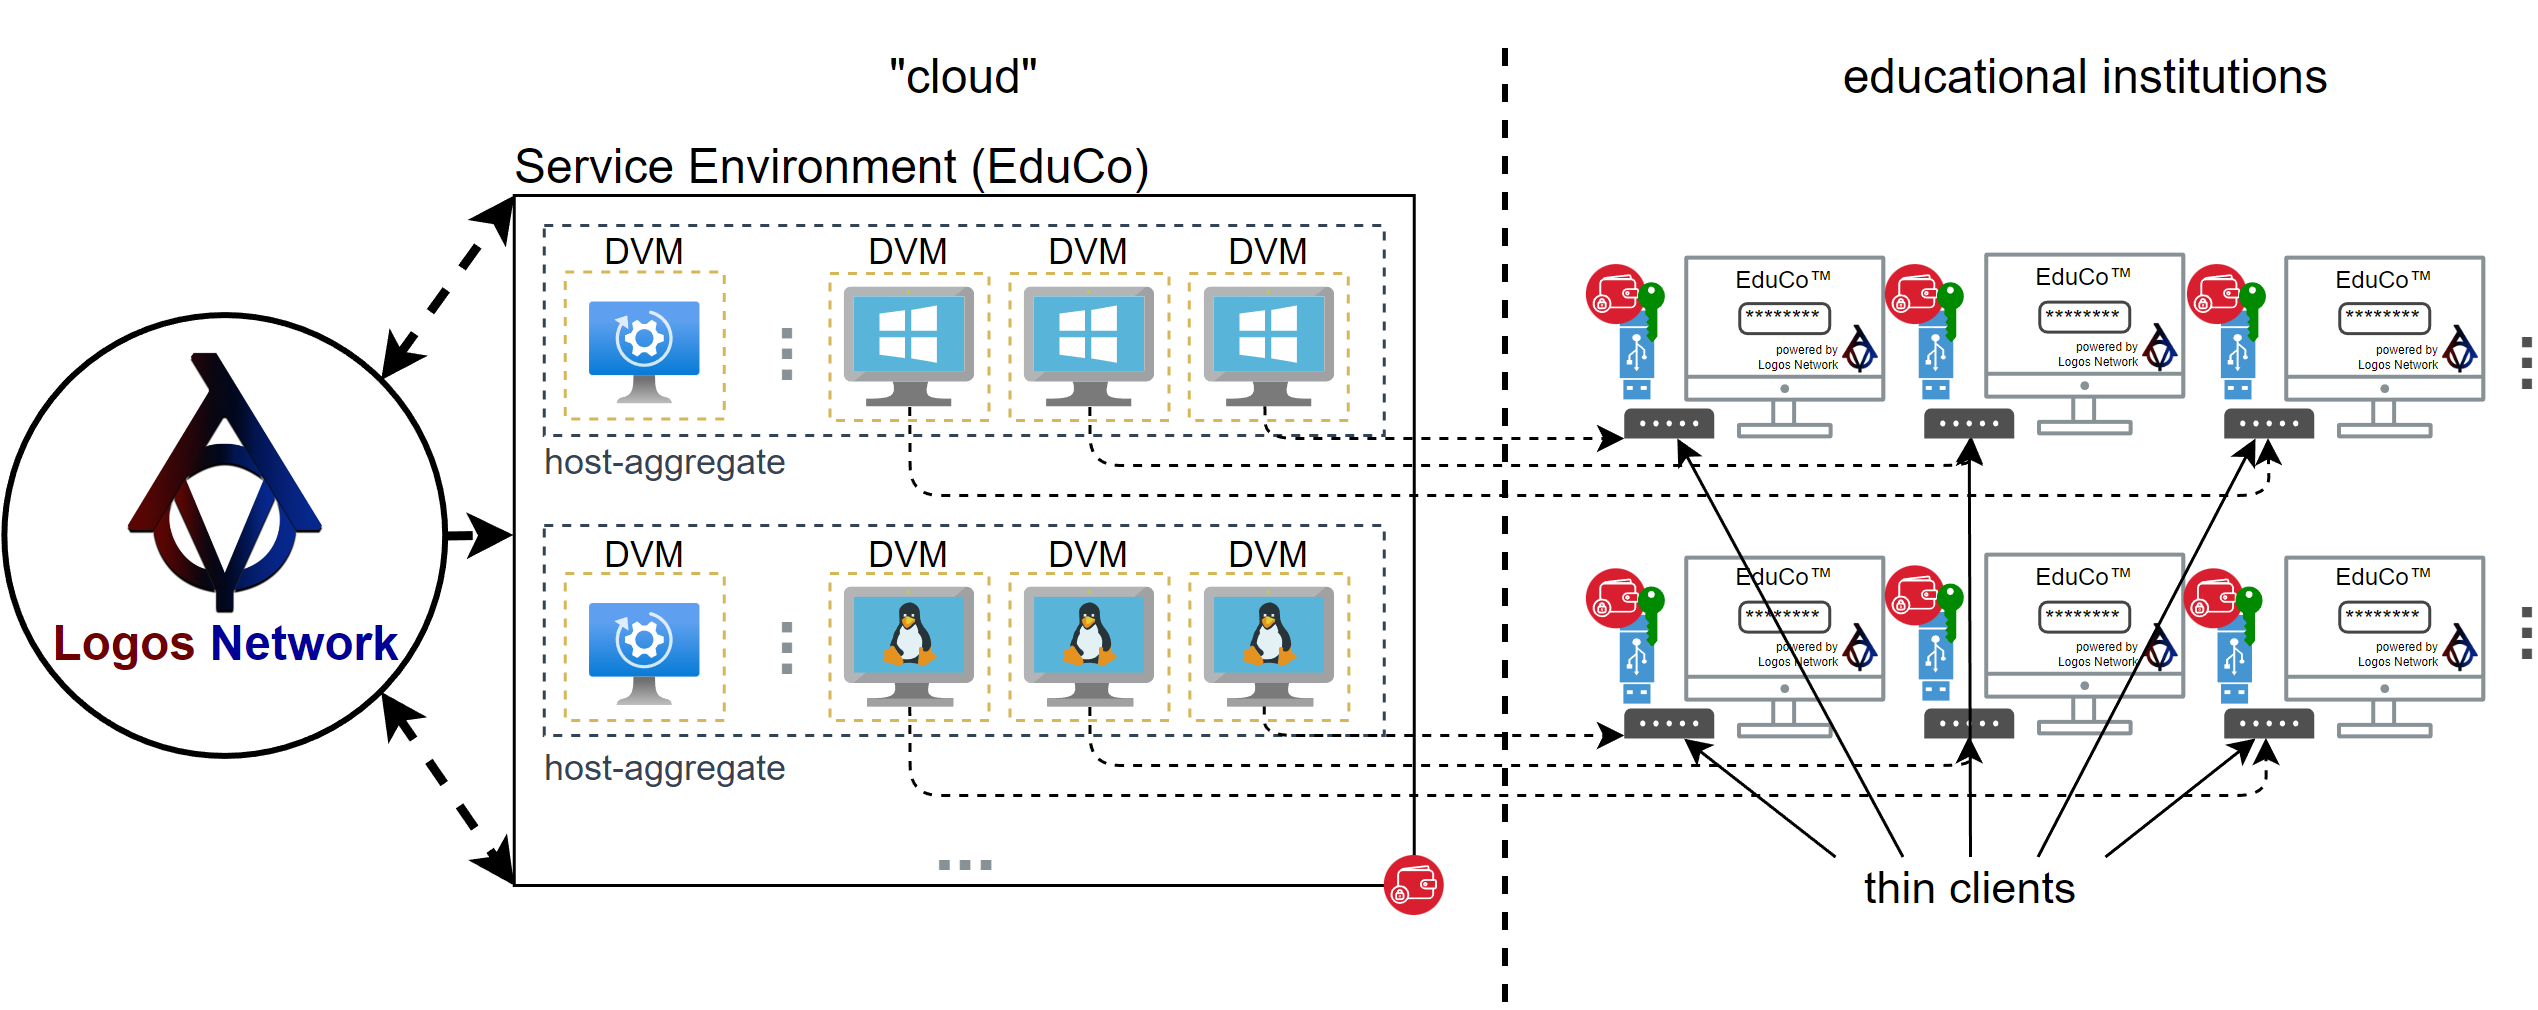
\includegraphics[height=5.7cm]{educo-overview}
\end{center}
\begin{center}
	Figure 16: High-level overview of the educational compute service EduCo
\end{center}

% SIGLE BOARD CLIENT
\subsubsection{Single board client}
A Single Board Client will be a computer solution based on a single circuit board (Single Board Computer (e.g. Raspberry Pi, Intel NUC, ARM-based sigle board clients, ...)) and will be utilized as a thin client for Virtual Desktop Infrastructure solutions.
This type of client will provide compactness, energy efficiency and lower costs compared to traditional desktop PCs or laptops.

In a VDI or remote desktop context, the Single Board Client will be used to establish a connection to a server running the actual desktop environments and applications. 
The SBC serves as a thin client that only sends the user interface and user input to the server and returns the server's output (such as the graphical display) to the user.

The SBC is to be developed by LogosLabs (in-house or outsourced) and should be specially designed for use by EduCo VDI solutions. 
Since the device will be only a remote client and the workstation (state of the art) will be in the cloud, it will not require an expensive device.

% SCICO
\subsection{SciCo}
SciCo will be the continuation of the EduCo service, provisioning the leased computational resources to scientific institutions. 
The main difference between those two services is, that the one (EduCo) uses the network resources to provide a cloud-workspace and the other (SciCo) utilizes same resources for complex scientific calculations (GPU-accelerated applications, Data Mining, Predictive computation, ...). 

% DISTRIBUTET COMPUTING
\subsubsection{Scientific computing platform}
The SciCo cloud platform will be a specialized online environment for scientific computing, designed to fulfill the requirements of scientific institutions and researchers. 
This platform will offer a range of features and resources specifically designed for complex scientific computing and data analysis.
It will provide researchers from computational scientific fields (comp. astrophysics, comp. geophysics, comp. forensics, ...) with access to computing resources (CPU and GPU).

Research institutions will be able to expand or decrease their computing capacities as required. 
This is particularly useful for projects that require different amounts of resources at different times.
Overall, such a platform should enable scientific institutions to perform their research more efficiently and more effectively by giving them access to computing resources without the need to maintain their own extensive IT infrastructure.

The design of a cloud platform for scientific computing that uses OpenCL and ROCm to utilize the resources of different GPUs will require a specific technical architecture, which will be described in detail in the technical documentation.
The platform will support two GPU types. (AMD and NVIDIA GPUs to ensure both OpenCL and ROCm compatibility).
The platform will provide several general features like GPU management and orchestration, data management and analysis, security and compliance, scalability and elasticity, ... . 
The Service will provide a user-friendly, web-based dashboard for accessing resources, monitoring tasks and managing projects, as well as providing APIs to enable integration with external systems and workflow automation.

Initially, there will be no provision of web-based IDEs or frameworks that support OpenCL and ROCm for the development of GPU-accelerated applications.
This feature may be re-evaluated in the future should there be a requirement. 

% FIGURE17
\begin{center}
	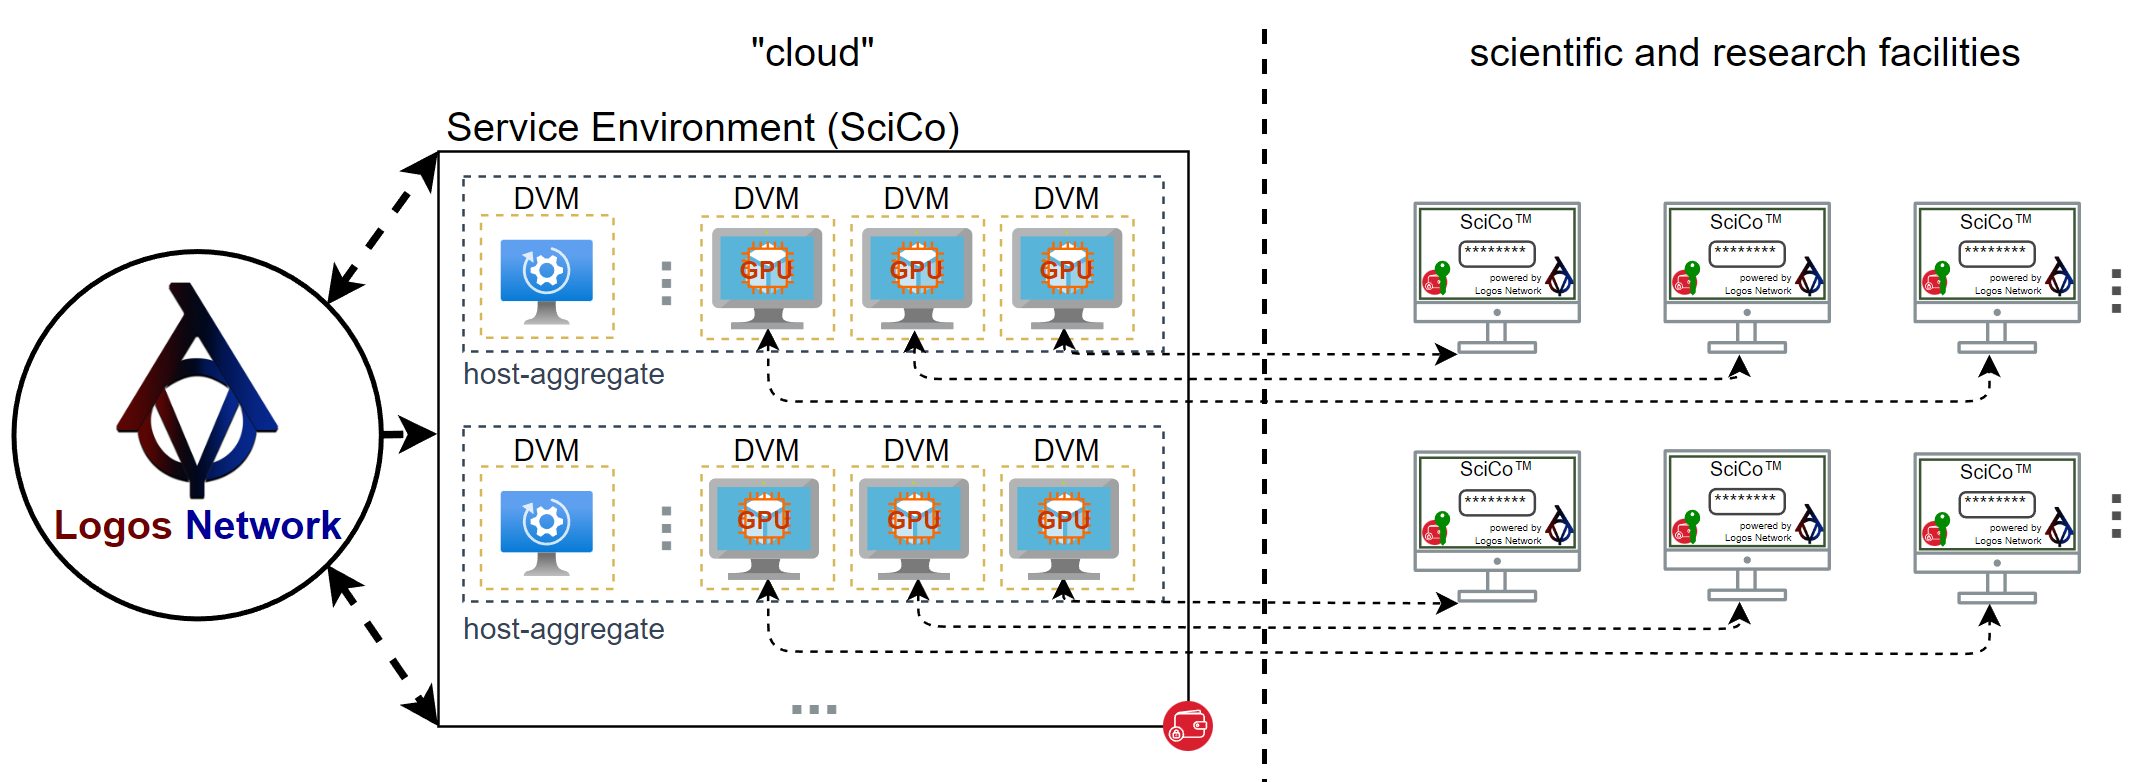
\includegraphics[height=5.4cm]{scico-overview}
\end{center}
\begin{center}
	Figure 17: High-level overview of the Science Computer a computational infrastructure for scientific applications;SciCo
\end{center}

Generally speaking, the aim is to create a powerful, cost-efficient and flexible cloud platform for scientific computing that is specifically geared towards the use of OpenCL and ROCm for GPU-intensive tasks. 
This platform will be able to efficiently support a wide range of scientific computations and data analysis, from bioinformatics to physics simulations.

It is important to underline, similarly to the EduCo service, that a web2 solution has been described here and that the platform (SciCo service) will be migrated to a layer-1 blockchain. 
The reason for this decision to provide another service as a web2 based service is to verify the integration solutions developed within the EduCo service.

% REFERENCES
\newpage
\printbibliography % usage: text \cite{key} # references
\newpage

% GLOSSARY
\section*{Glossary}
\addcontentsline{toc}{section}{\protect\numberline{}Glossary}    
\begin{longtable}{p{0.3\linewidth} p{0.1\linewidth} p{0.45\linewidth} p{0.1\linewidth}}
	\textbf{Name}&\textbf{Acronym}&\textbf{Description}&\textbf{Definition}\newline \\ \hline
	\endfirsthead
	\textbf{Name}&\textbf{Acronym}&\textbf{Description}&\textbf{Definition}\newline \\ \hline
	\endhead

Access validator (NG) & AV & The Access validator (NG) is responsible for the validation of incoming requests (Logos network). & 2.3 \\ %LINE-END
Computing environment & CoE & The DVCI-layer-2 or back-end phase takes on layer-specific actions in managing, connecting and securing the DVCI. & 2.1.1 \\ %LINE-END
Computational network & CoN & A low-latency software-defined network that enable internal networking in a DVCI. & 2.1.4 \\ %LINE-END
Configuration smart contract & CSC & This smart contracts store the DVCI configurations. & 2.2.3 \\ %LINE-END 
Client environment & ClE & This environment is the "execution-layer" for the DVCI and act as the access point for services. & 2.1.1 \\ %LINE-END
Dedicated root server & DRS & These servers are used for providing an OpenStack environment for the DVCI in a global region. & 2.1.1 \\ %LINE-END
Distributed Virtual \newline Computing Infrastructure & DVCI & A Web3 cloud infrastructure. & 2.1 \\ %LINE-END
Distributet virtual machine & DVM & VMs created in a DVCI host-aggregate. & 2.1.1 \\ %LINE-END
Distributed resource Node & DRN & Provider of distributed resources.  & 2.1.1 \\ %LINE-END
DVCI book (NG) & & Data-source for the Translator (NG). & 2.3 \\ %LINE-END
DVCI validator (NG) & DVCI-AV & The DVCI-AV (NG) process requests explicitly from the DVCI. & 2.3 \\ %LINE-END
Educational compute service & EduCo & A community based compute service for educational purposes & 3.1 \\ %LINE-END
Environment controller node & ECN & The ECN consists of an OpenStack controller node and the main network gatekeeper. & 2.1 \\ %LINE-END
Executor (NG) & & The Executor (NG) deliver requests to the blockchain. & 2.3 \\ %LINE-END
Global region & & Computational resources (DVCIs) divided into geographic (global) regions. & 2.1.1 \\ %LINE-END
Knowledge keeper (NG) & KK & The Knowledge keeper (NG) contains data regarding the smart contract logic. & 2.3 \\ %LINE-END
LogBox & & Single-board device (thin-client), capable of accessing the cloud workspace. & 3.2 \\ %LINE-END
Logos network & LN & Web3 computational infrastructure. & 2.0 \\ %LINE-END
Logos chain & LC & Substrate based smart contract infrastructure. & 2.2 \\ %LINE-END
Network gatekeeper & NG & Middleware for the Logos network. & 2.3 \\ %LINE-END
Network gatekeeper daemon & NGd & The daemon (NG) is the component responsible for security monitoring. & 2.3 \\ %LINE-END
OpenStack environment & & OpenStack (environment) is a comprehensive cloud-infrastructure solution. & 2.1.1 \\ %LINE-END
Operation smart contract & OSC & This smart contracts perform certain operations or execution logic based on the configuration smart contracts. & 2.2.3 \\ %LINE-END 
Region bridge network & RBN & Is a network architecture approach (concept) in which services from one global region can access resources from another global region. & 2.1.4 \\ %LINE-END
Region environments & RE & The term region is used as a collective term for layer-2 and layer-3. & 2.1.1 \\ %LINE-END
sub0layer & & A decentralized core computing environment acting as the underlying layer to a Web3 infrastructure(layer-0) & 1 \\ %LINE-END
Science computer & SciCo & Computational infrastructure for scientific applications. & 3.3 \\ %LINE-END
Service network & SeNe & This networks are virtual networks that are provided by the OpenStack network nodes (neutron service) & 2.1.4 \\ %LINE-ENN	
Service environment & SE & Environments that provided by the Logos network (computation utilization)  & 2.1 \\ %LINE-END
Sigle board client & SBC & A computer solution based on a single circuit board and its used as a thin client for VDI-solutions. & 2.3 \\ %LINE-END
Smart contract logic & SCL & Comprehensive set of smart contract`s, tasked with the execution of case specific instructions & 2.2.3 \\ %LINE-END
Supply smart contract & SSC & Contract type that defines and implement the network gatekeeper and W3bI on the chain & 2.2.3 \\ %LINE-END
Translator (NG) & TL & Generate a requests, in the required format (in form of a transaction) to trigger smart contracts, and forward it to the Executor (NG) & 2.3 \\ %LINE-END 
Web2to3 smart contract & W2t3SC & This contracts enables the automated integration of web2 based services on the Logos network. & 2.3 \\ %LINE-END  
Web3 infrastructure service & W3bI & Core service of the Logos network and the ecosystem that "host" blockchain nodes (layer-0 and layer-1) & 3.3 \\ %LINE-END

	\caption{Glossary for the Logos network}
\end{longtable}

\end{document}
